% !TeX spellcheck = en

\chapter{Evaluation}
\label{sec:eval}
Chapter describes the evaluation metrics and performed experiments, visualises prediction results.

\section{Goal of evaluation}
\label{sec:eval:goal}
The goal of model evaluation is an estimation of the generalisation accuracy of a model on future unseen data. This master thesis aims to evaluate whether RNN neural networks modification as LSTM, GRU and bidirectional variant are able to reduce the positional and rotation error for given look ahead time of 100 ms. This LAT is higher than normal acceptable latency in VR applications and even higher that measured M2P latency in cloud streaming platform presented in work \cite{serhan_cloud_streaming}. Since the successfully trained best evaluated model is intended to be build in the server infrastructure, the goal of evaluation is to find out how using of RNN model can reduce the positional and rotational error and thus improve the quality of delivered from cloud server VV content by calculating the proper future 2D image from volumetric data.  

To evaluate all described above models, a Python-based application used for training and processing of the records via HoloLens 6-DoF datasets. Below, the first Baseline model, the experimental setup and the evaluation metrics are discussed, before presenting the obtained results and discussing the limitations of evaluated models.

\section{Evaluation metrics}
\label{sec:eval:metrics}
Evaluation metrics are used to measure the quality of the predictions made by machine learning models. This thesis similar to work \cite{serhan_kalman} uses two of the most common metrics Mean Absolute Error ($MAE$) and root mean squared error ($RMSE$).

Mean Absolute Error ($MAE$): MAE measures the average error over the test sample of the absolute differences between prediction and actual observation without considering their direction. 
\begin{equation}
MAE= \frac{1}{n} \sum_{j=1}^{n} |y_j - y_{mean}|
\end{equation}

Root mean squared error ($RMSE$): RMSE measures the average magnitude of the error with square root of the average of squared differences between prediction and actual observation.

\begin{equation}
RMSE= \sqrt{ \frac{1}{n} \sum_{j=1}^{n} (y_j - y_{mean})^2}
\end{equation}
Both MAE and RMSE express average model prediction error in units of the variable of interest, both metrics can range from $0$ to $\inf$ and are indifferent to the direction of errors. They are negatively-oriented scores, which means lower values are better\footnote{https://medium.com/human-in-a-machine-world/mae-and-rmse-which-metric-is-better}. Since the errors in $RMSE$ are squared before they are averaged, the RMSE gives a relatively high weight to large errors. Normally, The $RMSE$ result will always be larger or equal to the $MAE$. 

For calculation the metrics for positional data the Euclidean distance (L2 norm) is used.  Rotational metrics calculated with a distance between quaternions represented as an angle between their 3D orientations using a formula:
\begin{equation}
angularDistance = 2*arccos(real(p*conj(q)))
\end{equation}
where $p$ and $q$ are unit quaternions representing two rotations in the same basis and $q*$ denote the quaternion conjugate.

\section{Baseline model}
\label{sec:eval:baseline}
To understand how an evaluated model predicts and helps to reduce the M2P latency, some essentially a simple model that acts as a reference in a machine learning project must be implemented first. A Baseline model can lack complexity and may have little predictive power. The LSTM and GRU model should predict much better than a Baseline model and thus by comparing the metrics it can be understood how reasonable it is to implement and use the chosen approach. It is intended to use a Baseline model as benchmarks for trained models. There is no rule for what is a good or bad model's prediction. The criteria of model evaluation depends on the dataset and use case. A mean square error gives a value in units of the original dataset. For example, if a model predicts the prices of apartments in Berlin, then MAE of 1000 is a very good result and market's players would desire to have a trained model to work on the real estate market. However, it is abysmal for a model that predicts the price of average lunch in Berlin's restaurant. Thus a simple predictor is needed to predict future data so that predicted values can be compared with the real values using the same evaluation metrics as is used for RNN models.

The Baseline in this thesis is similar to the reference model used in the work \cite{serhan_kalman} and represents the operation of the system without prediction. It is assumed that the prediction time is set equal to the M2P latency of 100 ms such that the prediction completely eliminates the latency. Implemented Baseline is a deterministic model, meaning that it produces an expected output given the same input. For LAT of 100 ms a prediction time N is equal to 20 samples. The position and rotation data $x_t$ is simply propagated N samples ahead in the Baseline prediction and set as the user position and rotation at time $x_t + N$, i.e. $Baseline(x_t) = x_{t+N}$. 
\begin{figure}[htb]
	\begin{center}
		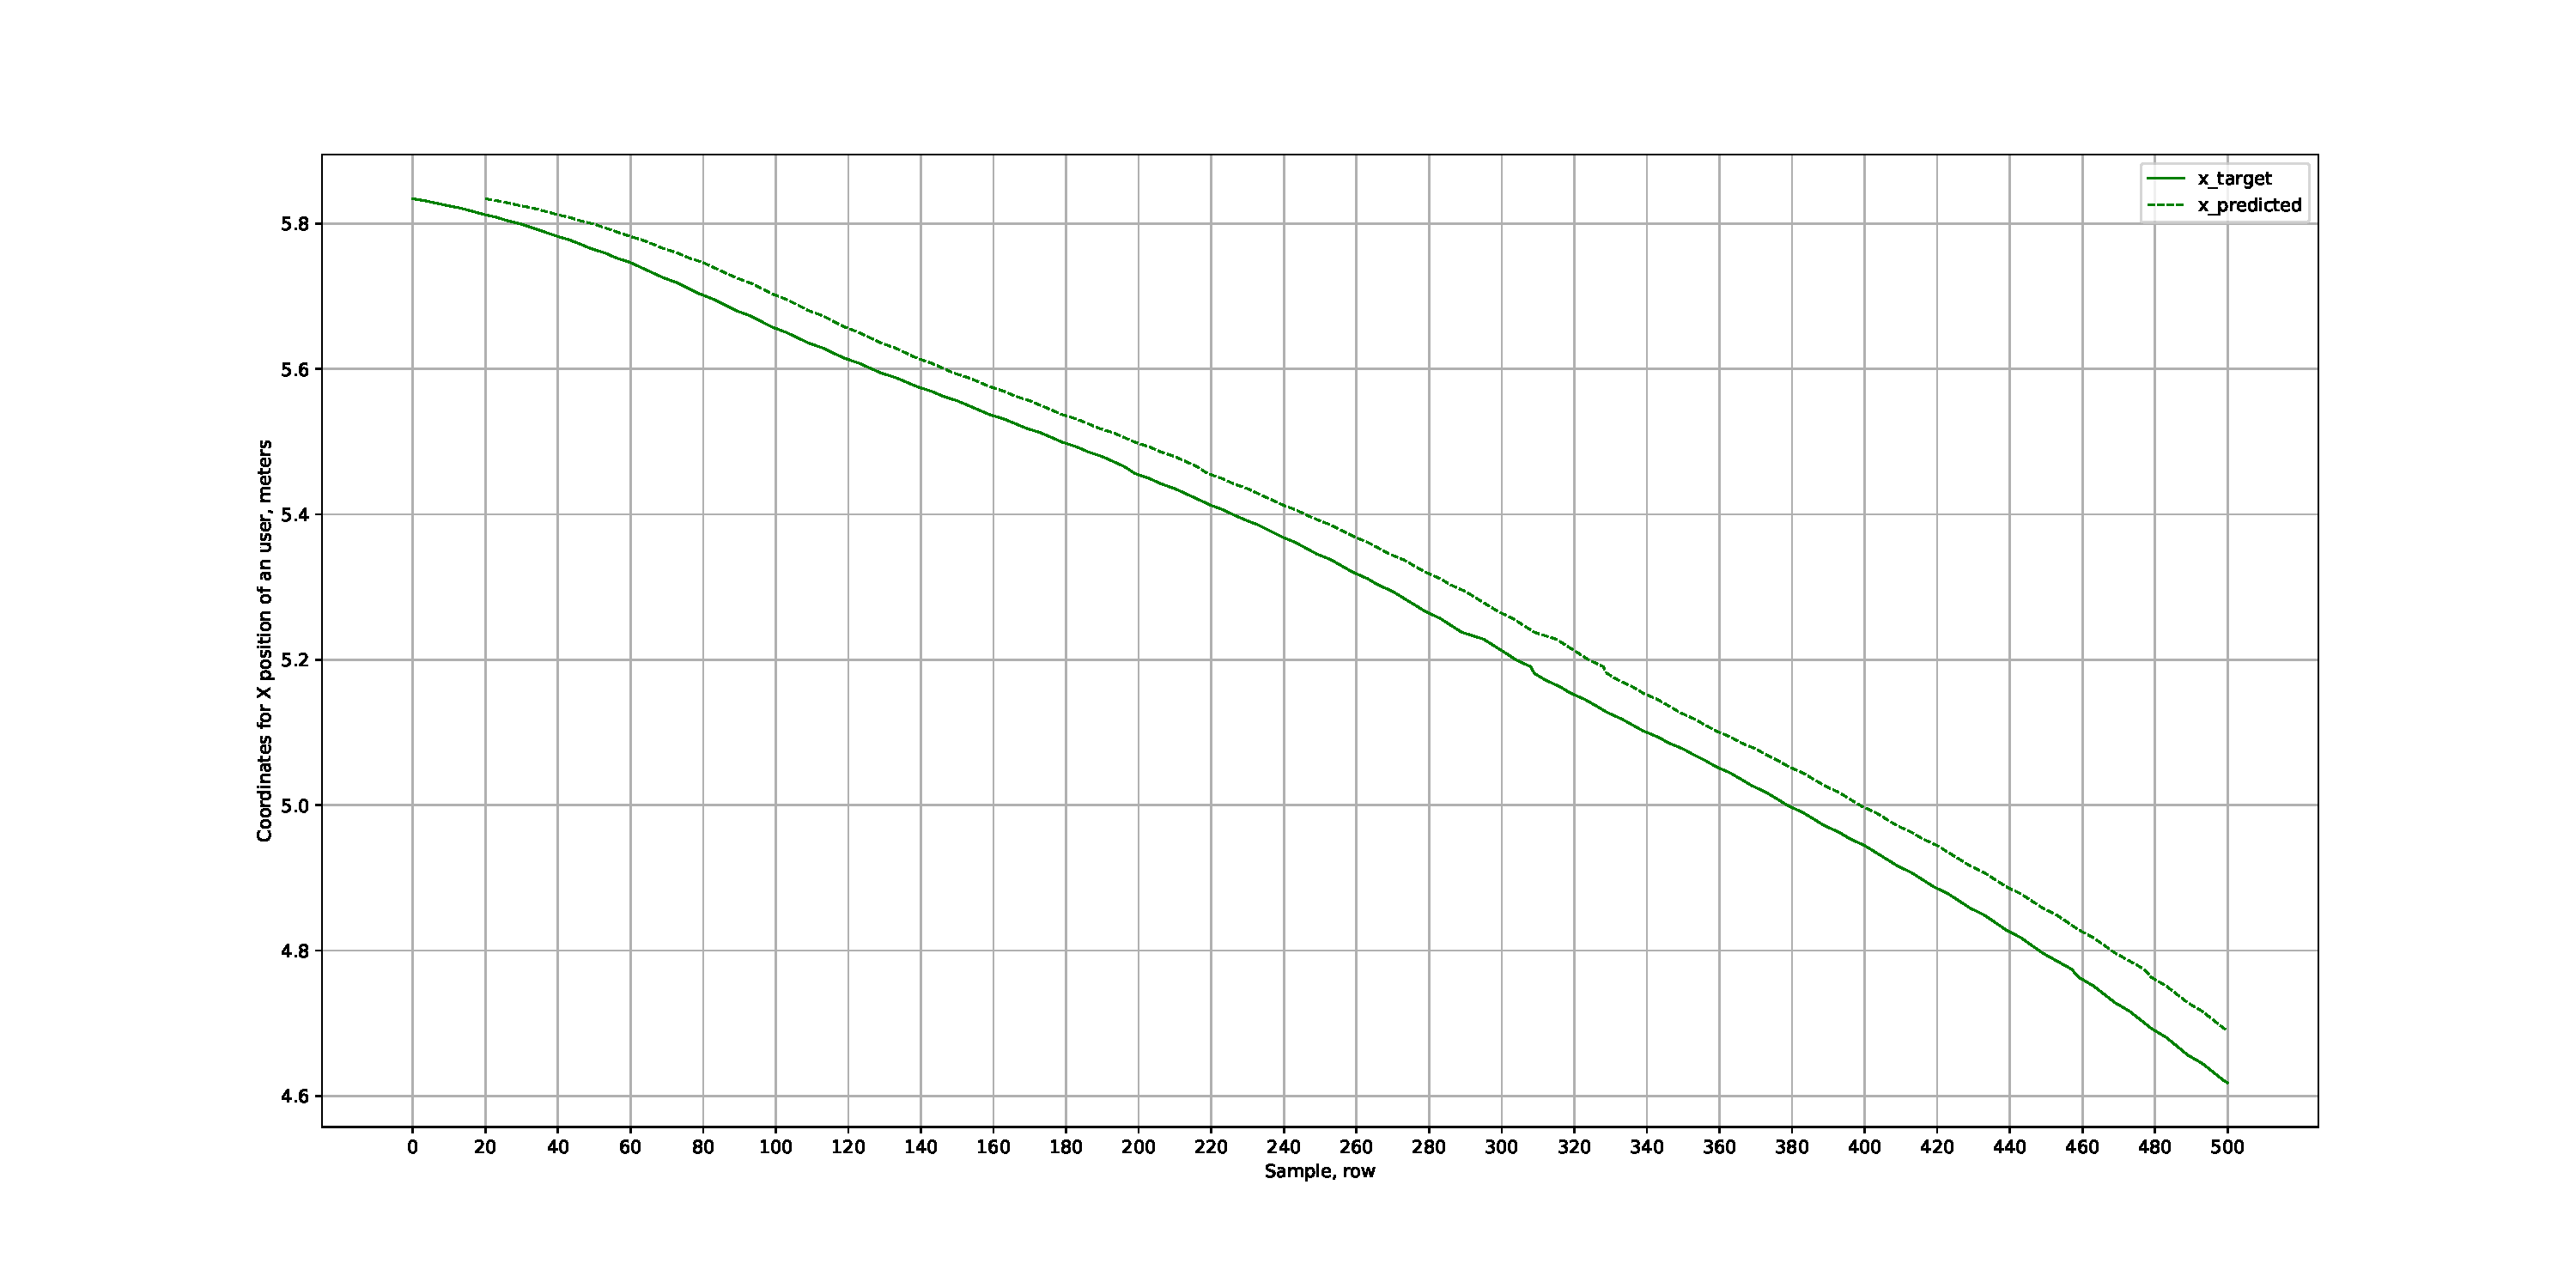
\includegraphics[width=1\textwidth, keepaspectratio]{gfx/base_zoom-x.pdf}
		\caption{\label{fig:base_x} Outputs of Baseline Model for x-axis.}
	\end{center}
\end{figure}

The Fig. \ref{fig:base_x} shows the first 500 real values and the corresponding output of the baseline for positional axis $x$. From the plot of the Baseline model outputs, it is clear that the model is 20-step behind reality. It copies with a given delay the falling trend and all fluctuations of the given axis.

The Fig. \ref{fig:base_xyz} shows the 500 real values and the corresponding output of the baseline for all three positional axes $x, y, z$. The plot samples 500 elements starting from the 2500 row and thus no missing data is seen on Baseline output for the first 20 elements as it is plotted in Fig. \ref{fig:base_x}. However, the Fig. \ref{fig:base_xyz} highlights the limitations of the usage of naive predictor that will deliver 2D image created from volumetric video content with a delay of 100 ms that is unappropriated delay for a human to experience in VR application without physical consequences like motion sickness \cite{delay_sickness}. The mean square error for the all three positional axes $MAE_{pos} = 0.067$m and root mean square error  $RMSE_{pos} = 0.068$m meaning the average distance between predicted position and the real position is equal to almost 7 cm. It is not crucial when a user looks at the big VV object, like a volumetric human hologram, from a distance of 3-4 metres. But if a user interacts with the small VV objects presented in the VR environment, then this distance becomes a significant difference between what user will see with a delay and where the VR object would be placed for delayed position.

\begin{figure}[htb]
	\begin{center}
		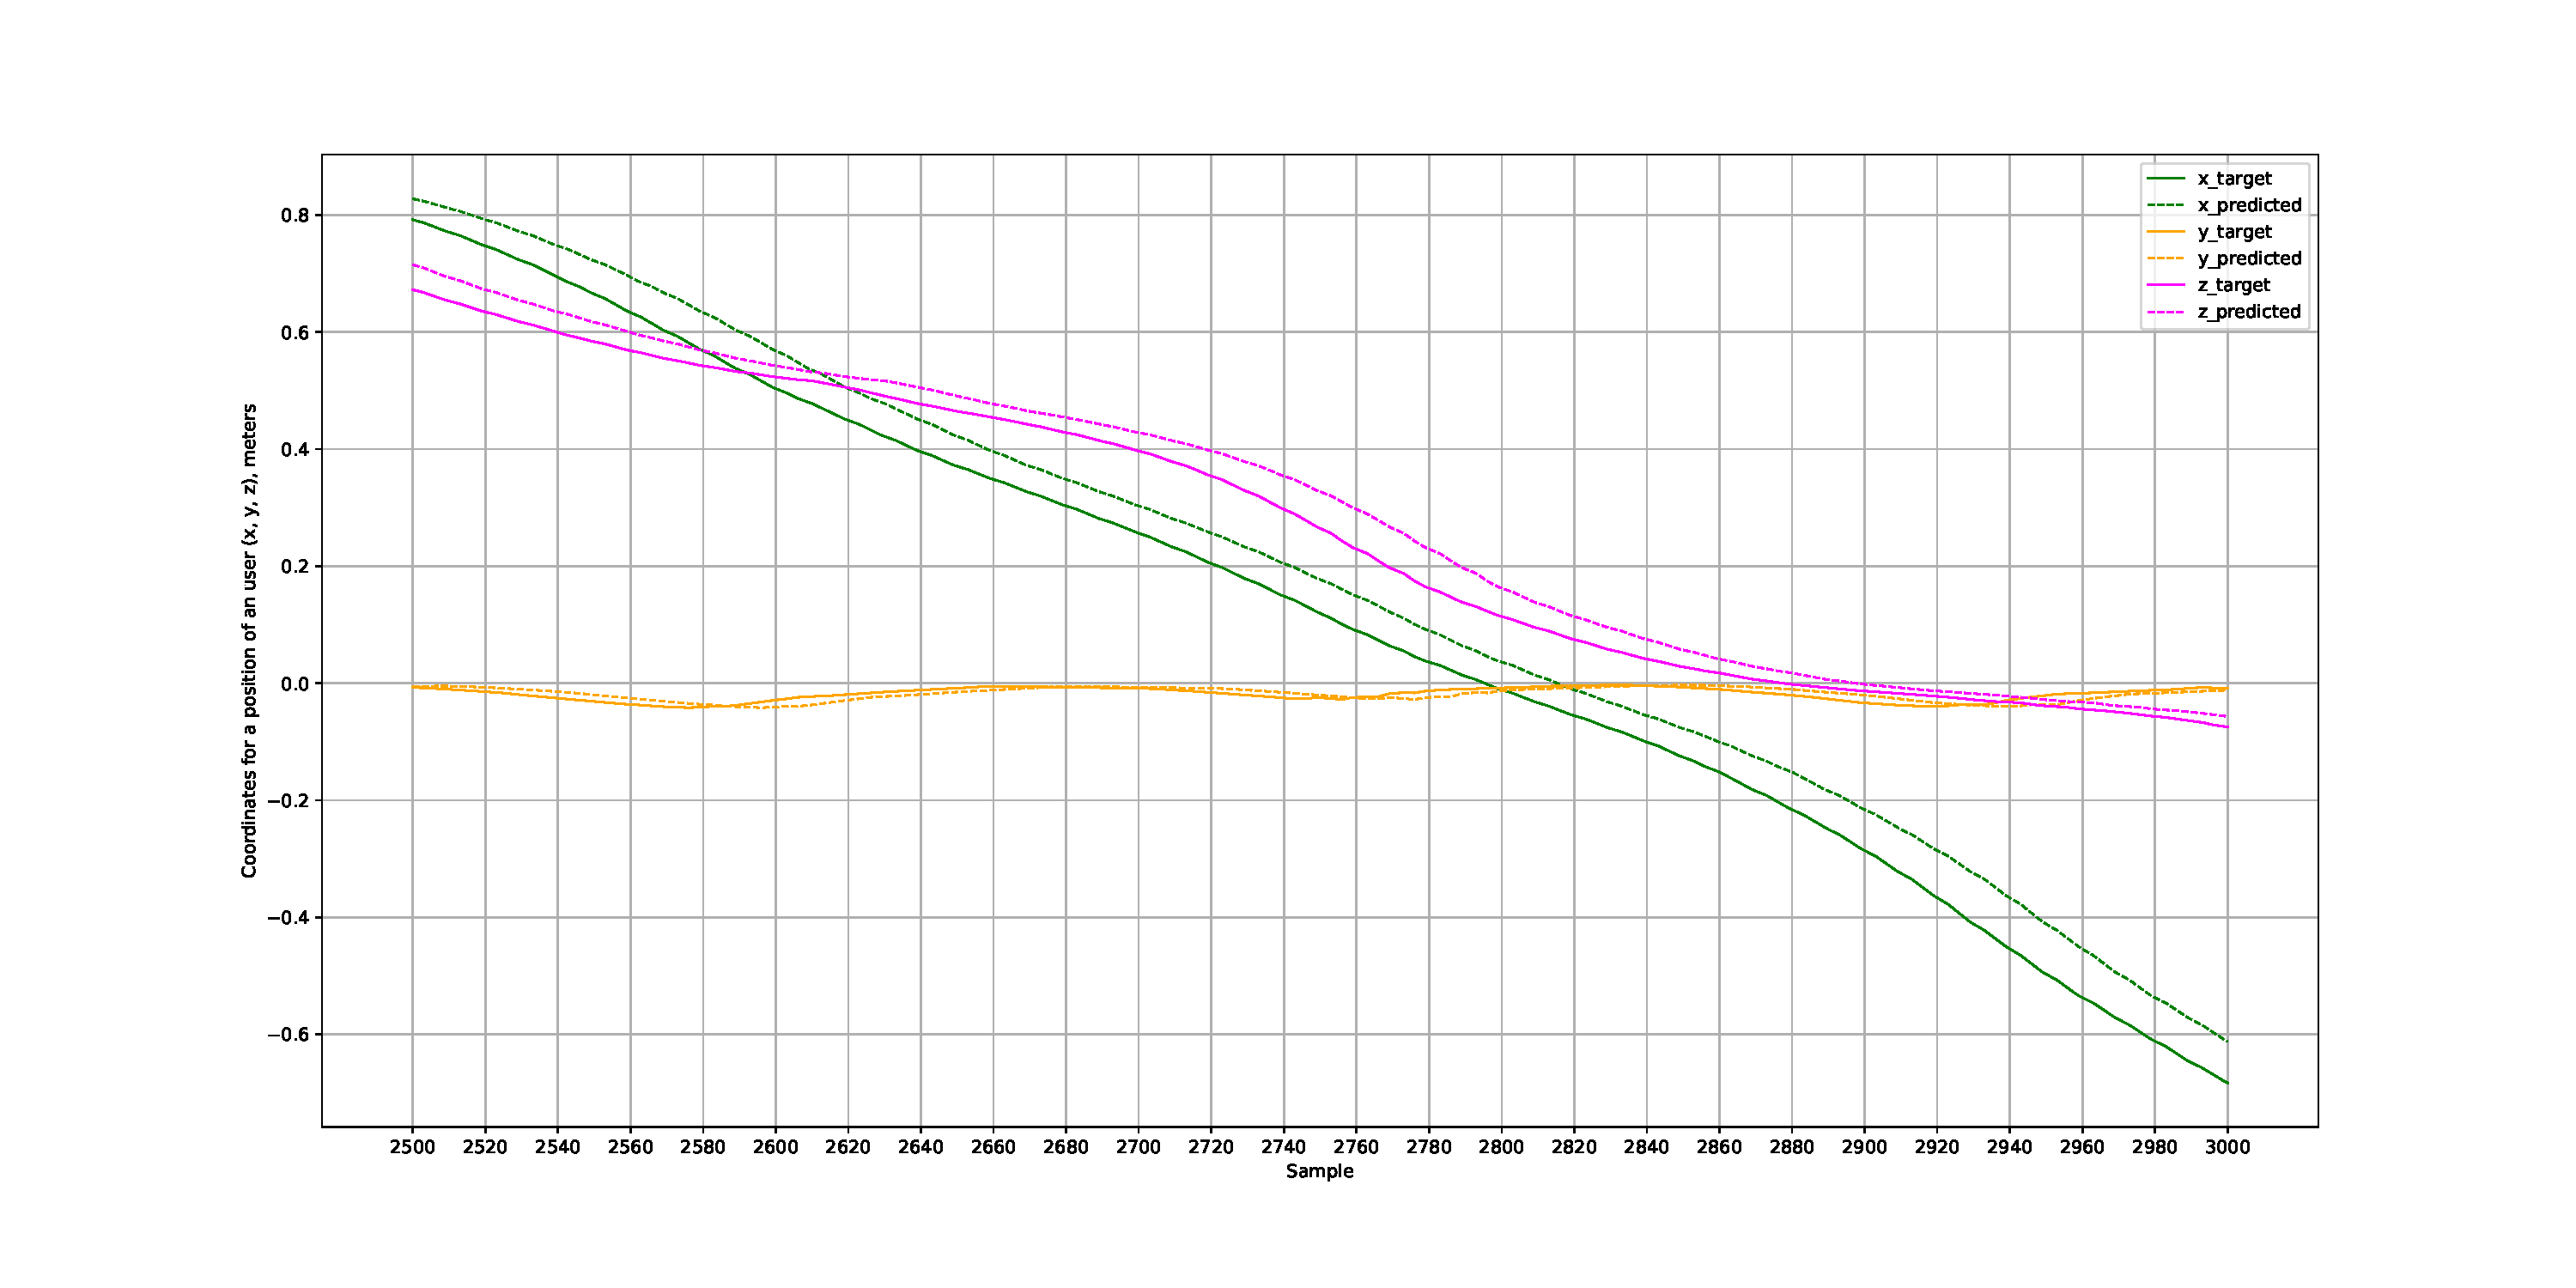
\includegraphics[width=1\textwidth, keepaspectratio]{gfx/base_zoom-xyz_position.pdf}
		\caption{\label{fig:base_xyz} Outputs of Baseline Model for x, y and z axes.}
	\end{center}
\end{figure}

It is worth to mention that in the case if real data is neither increasing nor decreasing in the given interval and fluctuates near the constant value, as it seen at $y$-axis, than the delay of the Baseline output is more not obvious when visualised due the overlapping of two graphs. In fact, the Baseline outputs have the same delay as those with good visualised delay as, for example, $x$-axis.

Fig. \ref{fig:base_quat_xyzw} shows the Baseline outputs for quaternions components $qx, qy, qz$ and $qw$. Same as with positional data, the same delay of 20 samples is present on rotational data. For all four quaternion components calculated metrics  are: $MAE_{rot} = 14.61^{\circ}$ and $RMSE_{rot} =21.24^{\circ}$.  

\begin{figure}[htb]
	\begin{center}
		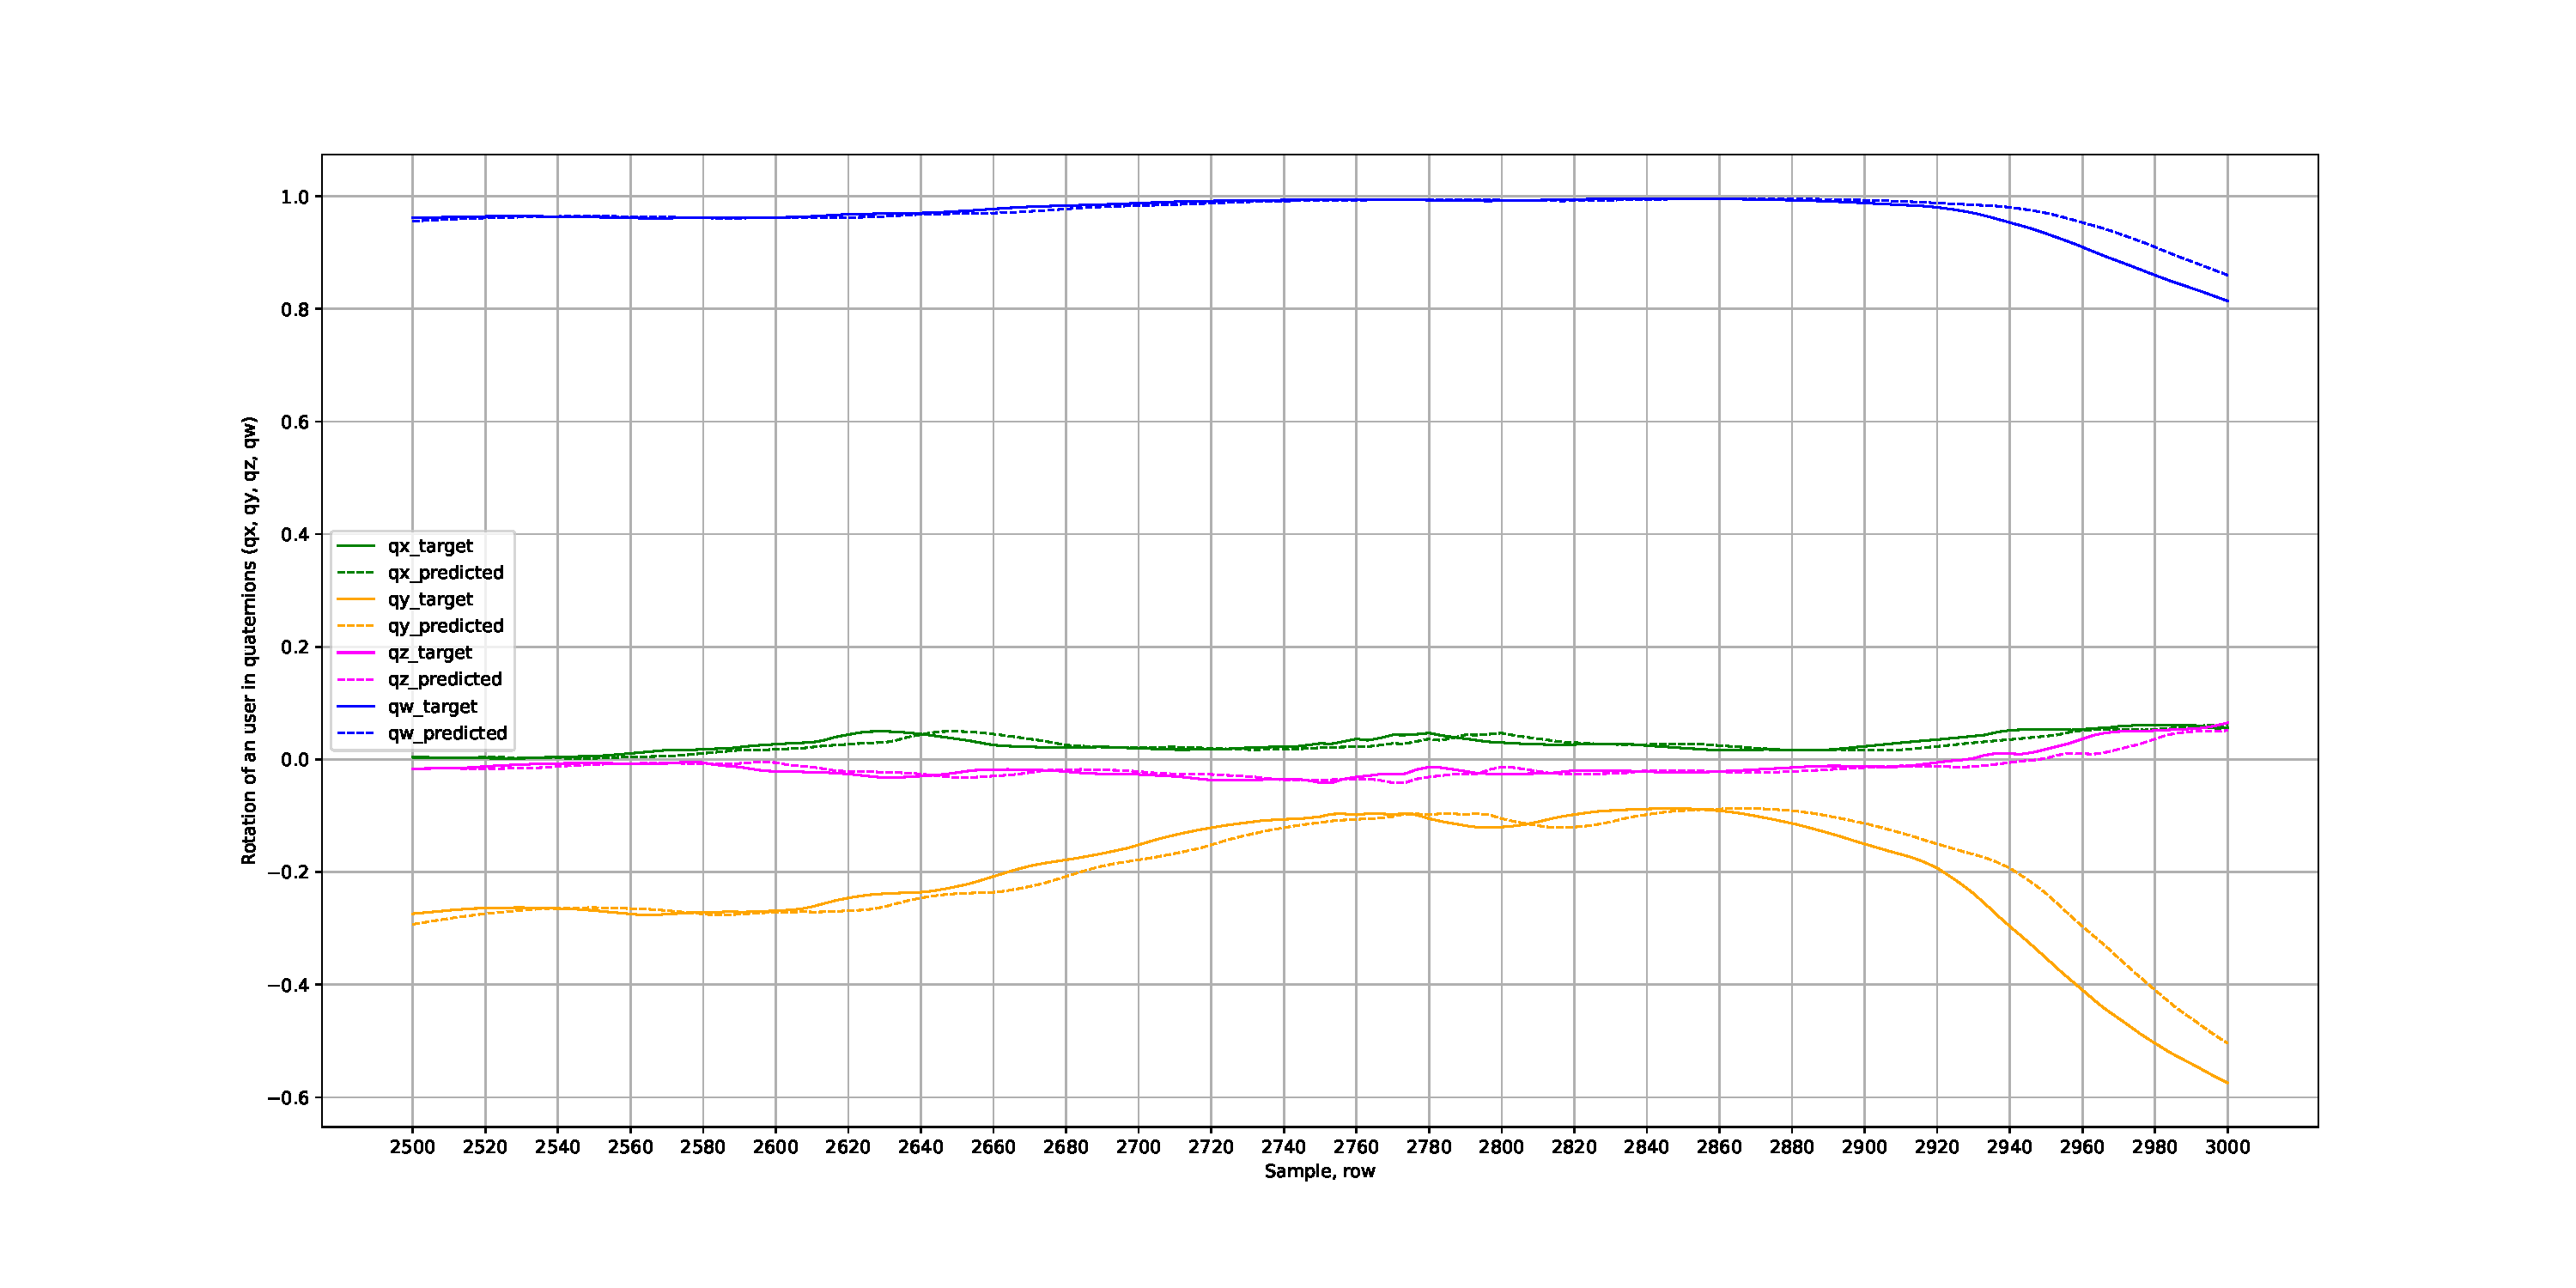
\includegraphics[width=1\textwidth, keepaspectratio]{gfx/base_zoom-qx_qy_qz_qw_rotation.pdf}
		\caption{\label{fig:base_quat_xyzw} Outputs of Baseline Model for quaternions components qx, qy. qz and qw.}
	\end{center}
\end{figure}

Because metrics of rotational data are measured in degrees, for visualisation purposes, orientations are given in the Fig. \ref{fig:base_euler} as Euler angles (yaw, pitch, roll), although prediction is performed in the quaternion domain.

\begin{figure}[htb]
	\begin{center}
		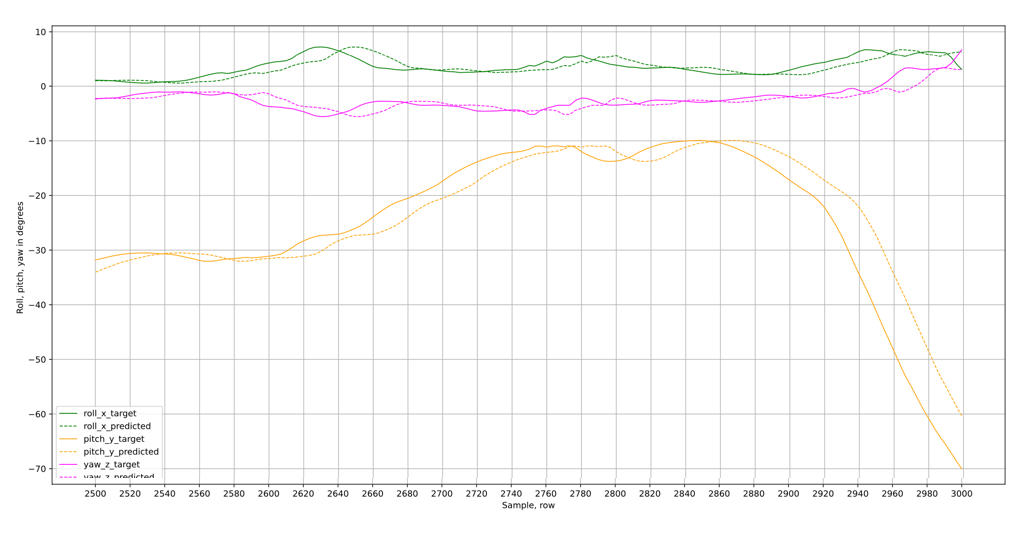
\includegraphics[width=0.85\textwidth, keepaspectratio]{gfx/base_euler-roll_pitch_yaw.png}
		\caption{\label{fig:base_euler} Outputs of Baseline Model for rotation data represented as Euler angles.}
	\end{center}
\end{figure}

The evaluated RNN model is considered to be successfully trained if the $MAE$ and $RMSE$ metrics at least for positional or rotational data can show significant improvement comparing to a Baseline output. 

\newpage
\section{Experiments}
\label{sec:eval:experiments}
In the experiments implemented models were trained with different hyperparameters and evaluated using $MSE$ and $RMSE$ metrics. 

\subsection{First experiments}
\label{sec:eval:experiments:early}

\subsubsection{Datasets}
\label{sec:eval:experiments:early:ds}
This section describes the difference of prediction results done by a model LSTM1 on different types of 6-DoF datasets. As already stated in section \ref{sec:impl:dataset:preprocessing}, original row dataset is not used in model training and was preprocessed before training was started. The following dataset were created and tried:

\begin{itemize}
	\item \textbf{Interpolated dataset:} Row dataset was interpolated so that missing values were inserted with linear interpolation for positional data and spherical linear interpolation for rotational data. 
	\item \textbf{Flipped dataset:} Interpolated dataset with flipped negative quaternions so that neighbouring quaternions are representing same rotation without significant 4D vector space between them
	\item \textbf{Normalised dataset:} Feature scaling (Min-max normalisation) is applied on the dataset's positional values to scale data in the range [0..1]. 
	\item \textbf{Position:} Only positional data $(x, y, z)$ as separate dataset to predict future position. 
	\item \textbf{Rotation:} Only rotational data $(qx, qy, qz, qw)$ as separate dataset to predict future rotation. 
	
\end{itemize}

% !TeX spellcheck = en

\begin{figure}
	\begin{center}
		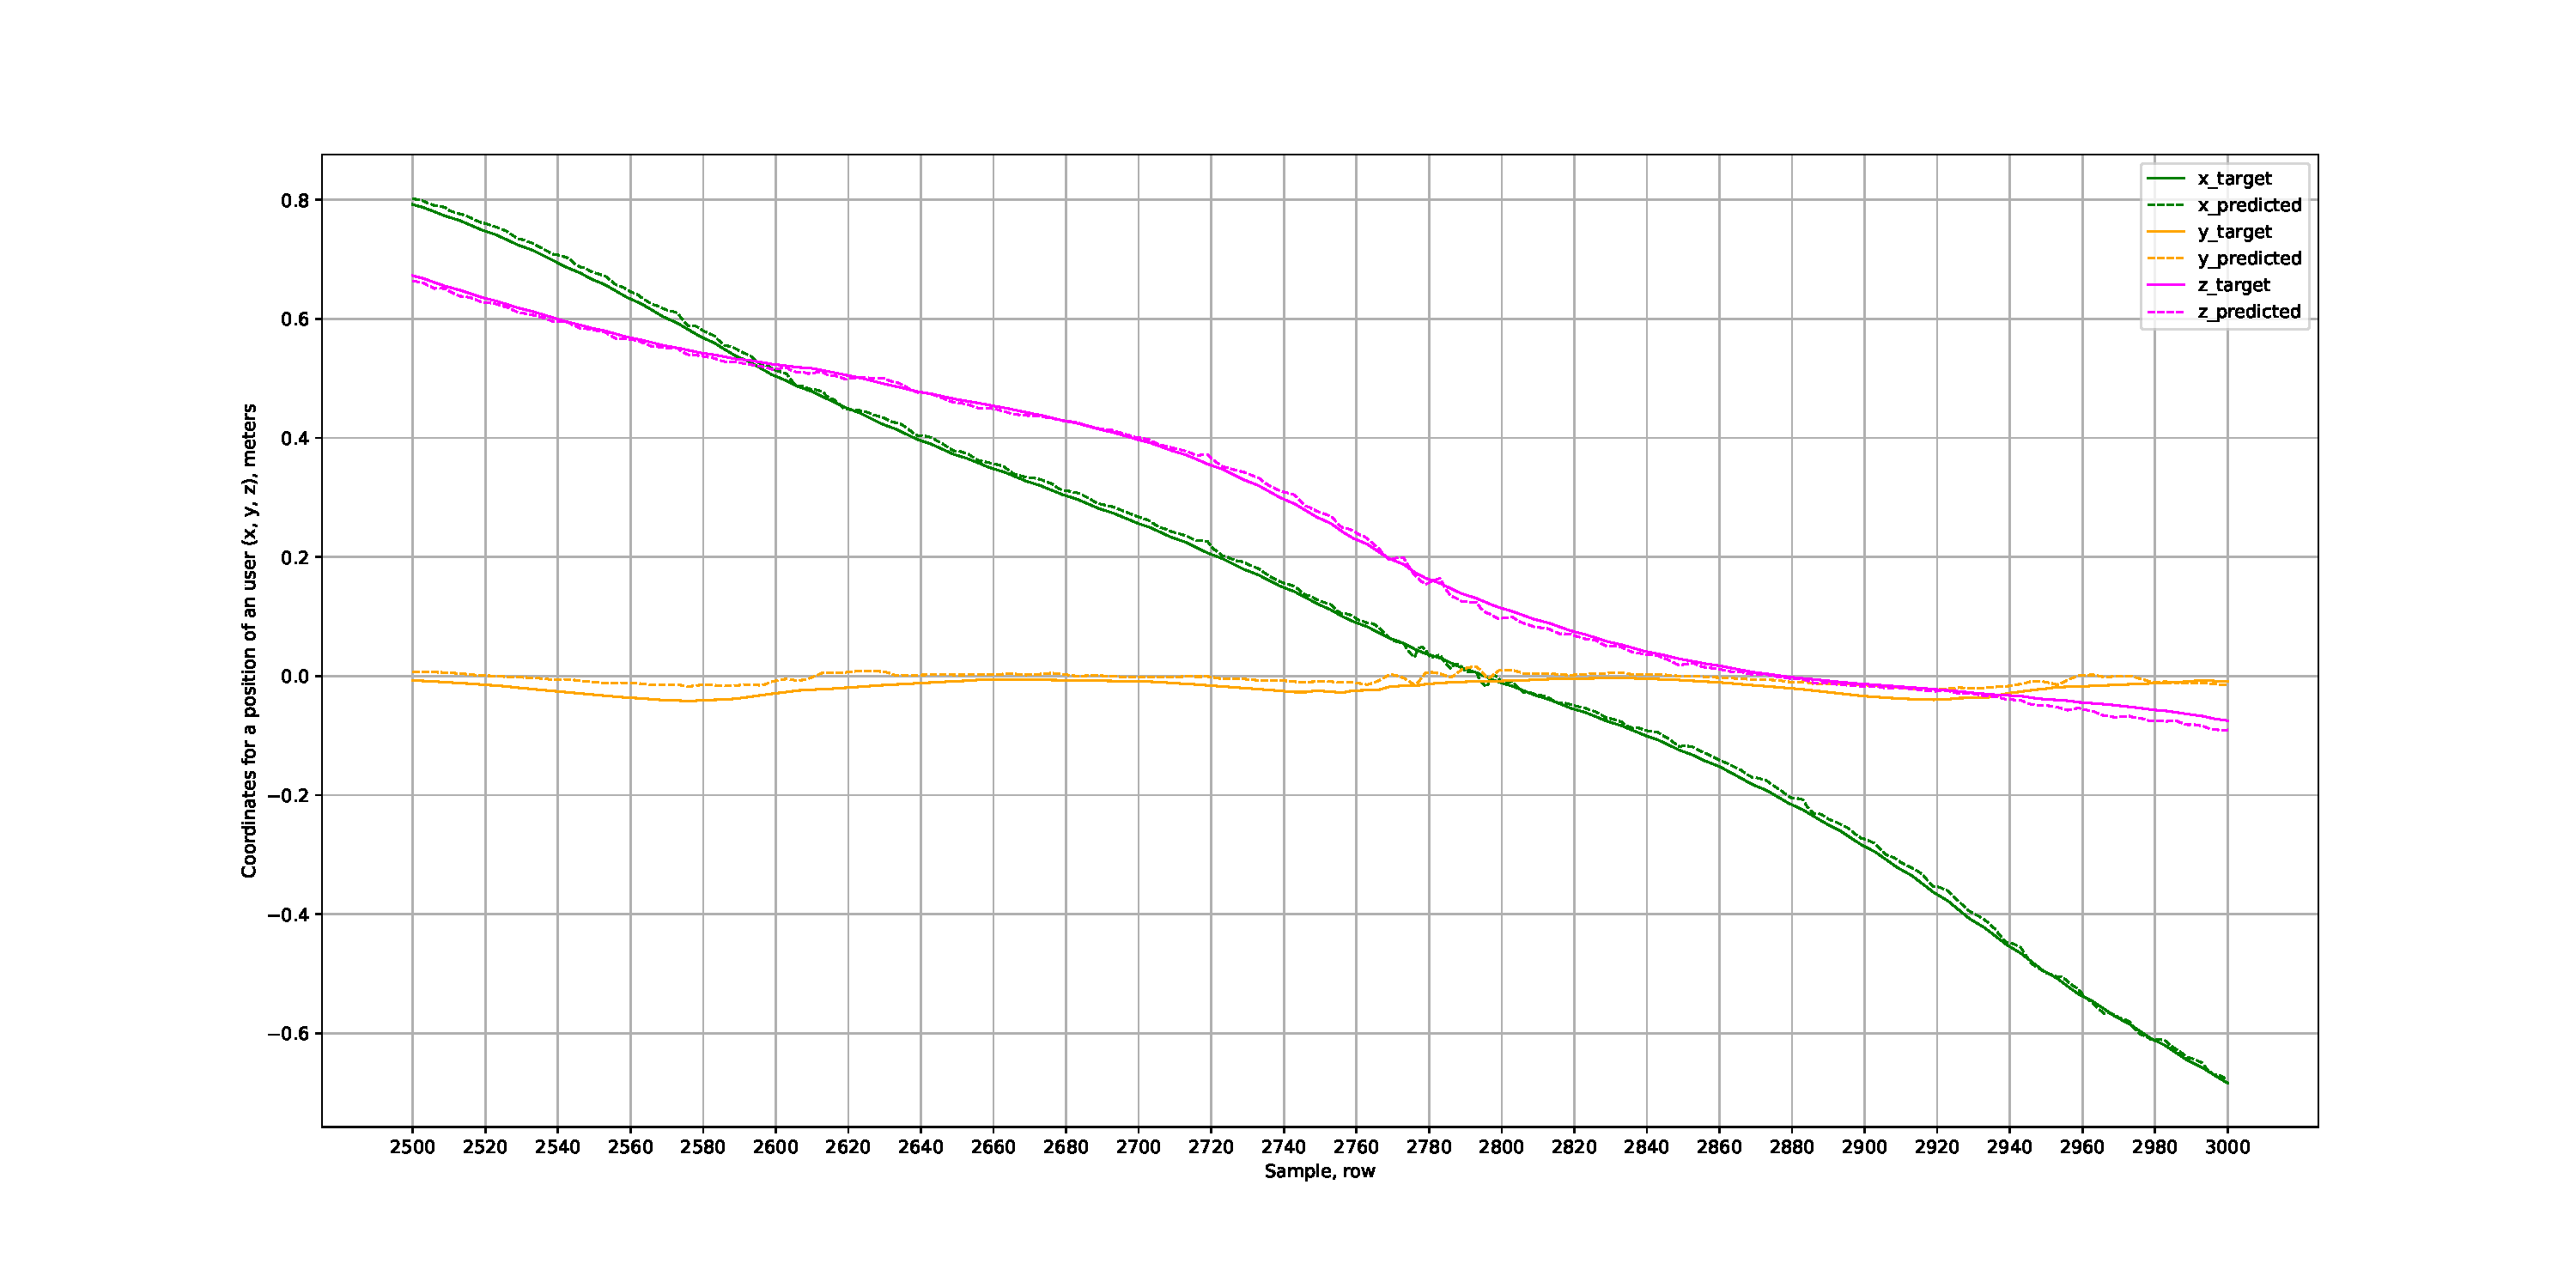
\includegraphics[width=0.9\textwidth, keepaspectratio]{gfx/lstm1_interpolated-xyz_position.pdf}
		\caption{\label{fig:interp1} Outputs of LSTM1 model on interpolated dataset for x, y and z axes.}
	\end{center}
\end{figure}

\begin{figure}
	\begin{center}
		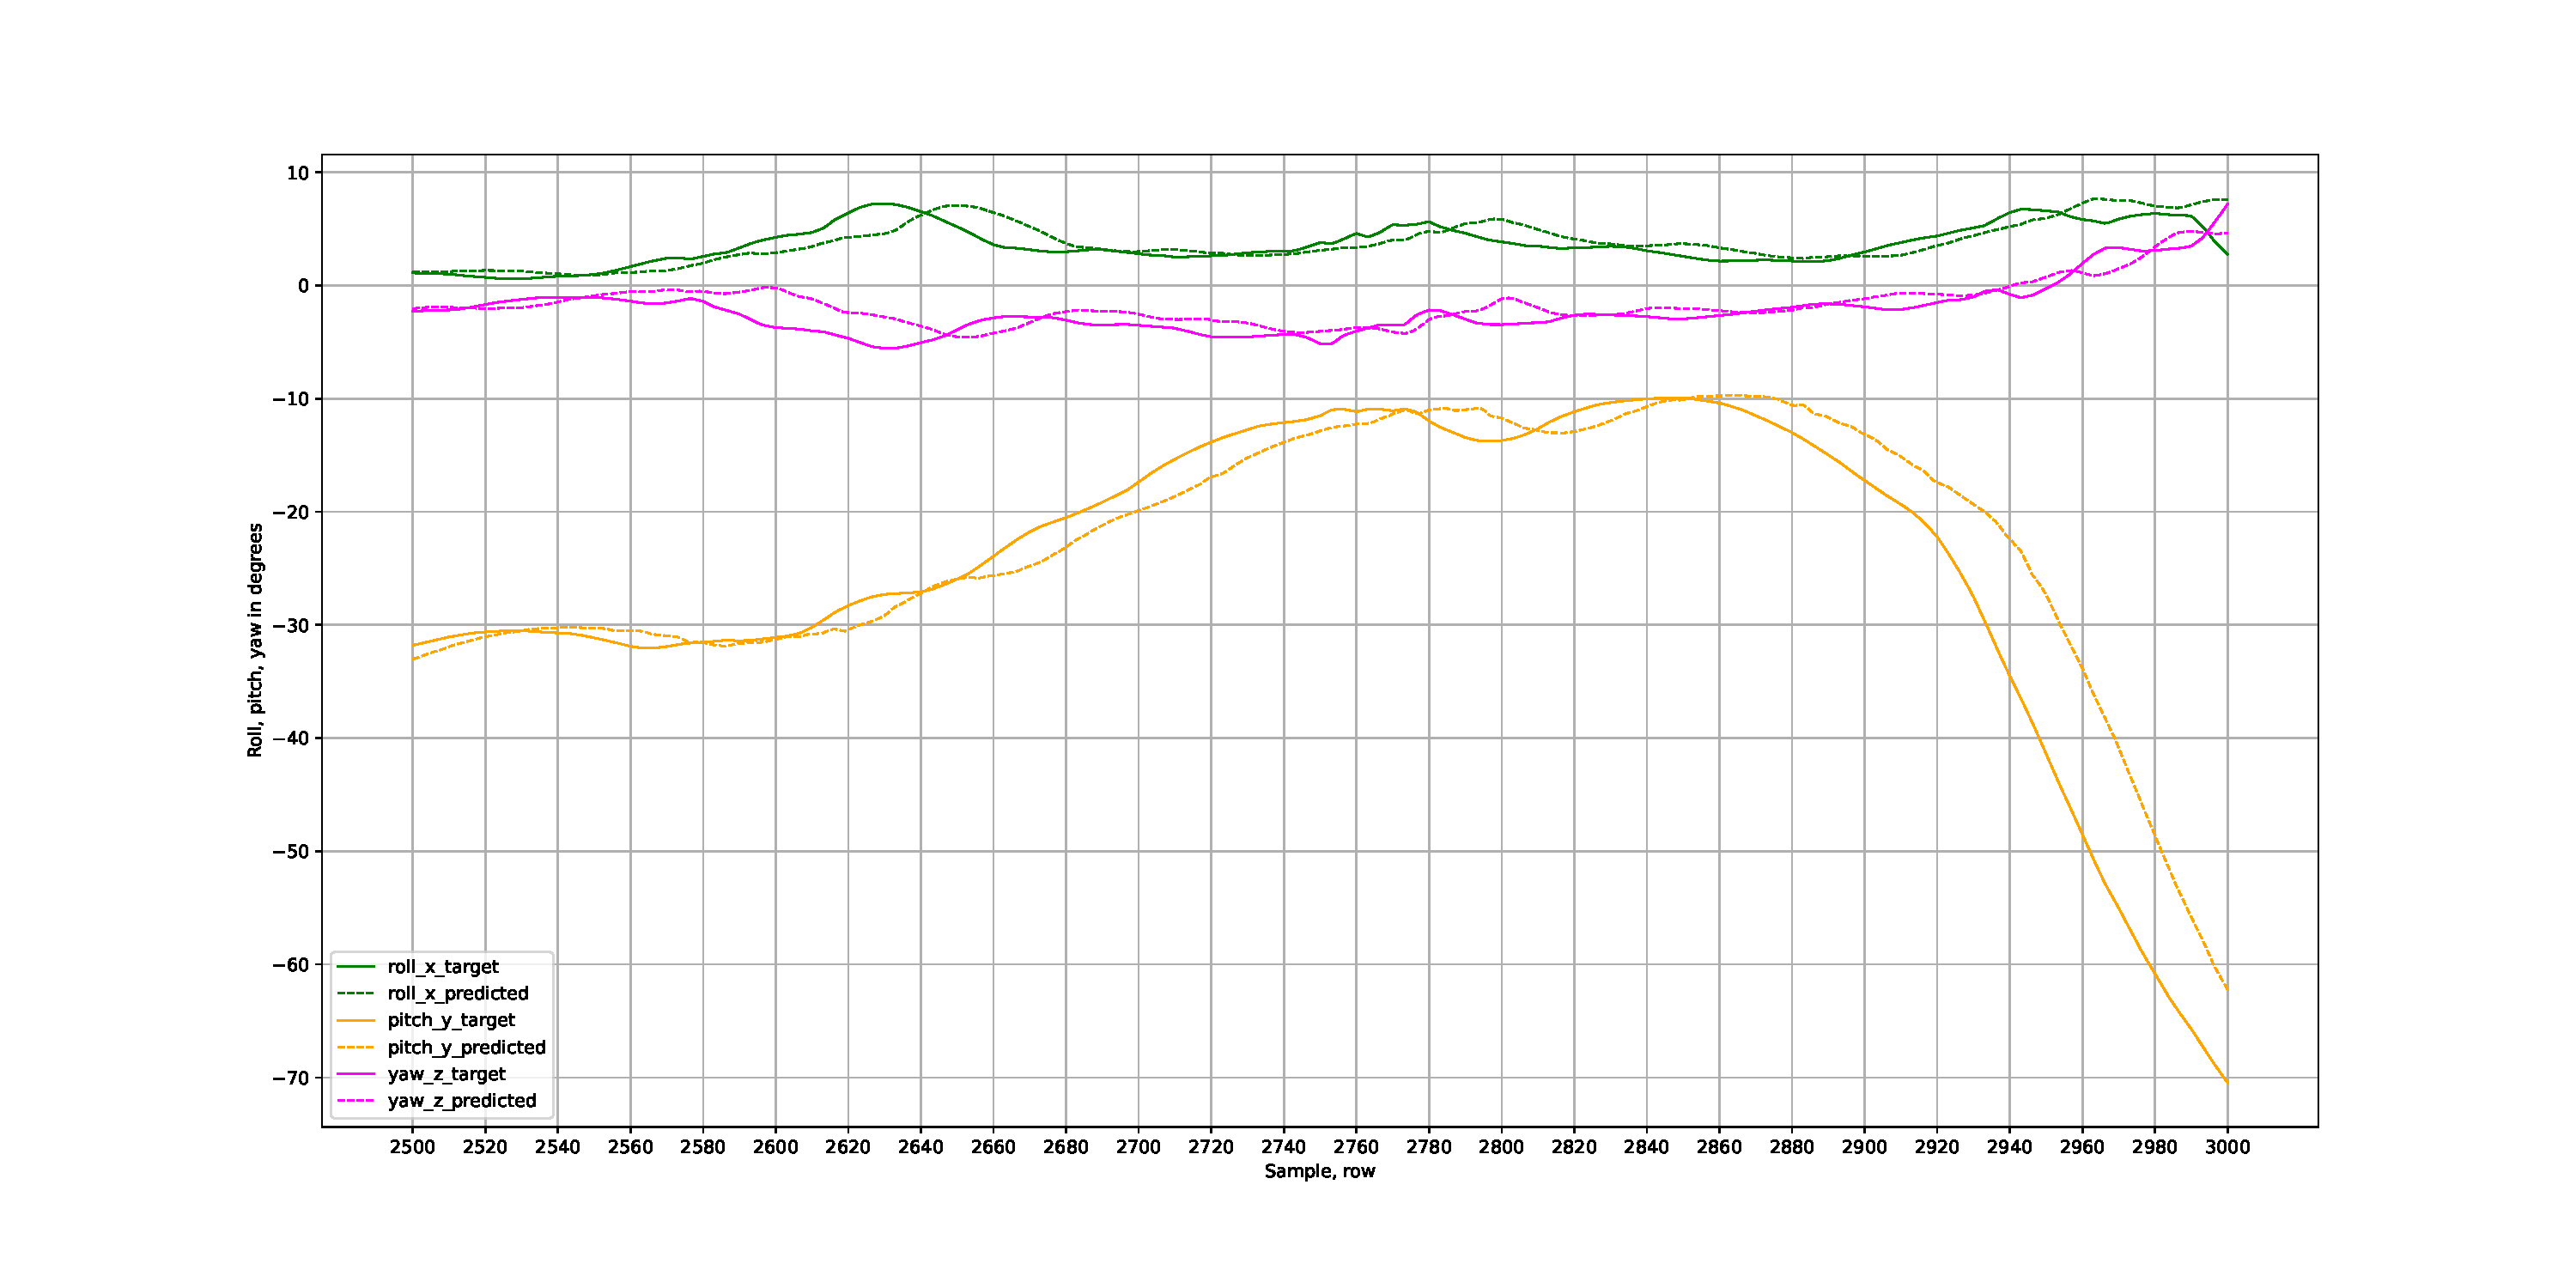
\includegraphics[width=0.9\textwidth, keepaspectratio]{gfx/lstm1_interpolated-roll_pitch_yaw.pdf}
		\caption{\label{fig:interp2} Outputs of LSTM1 model on interpolated dataset for roll, pitch, yaw axes.}
	\end{center}
\end{figure}

\begin{figure}
	\begin{center}
		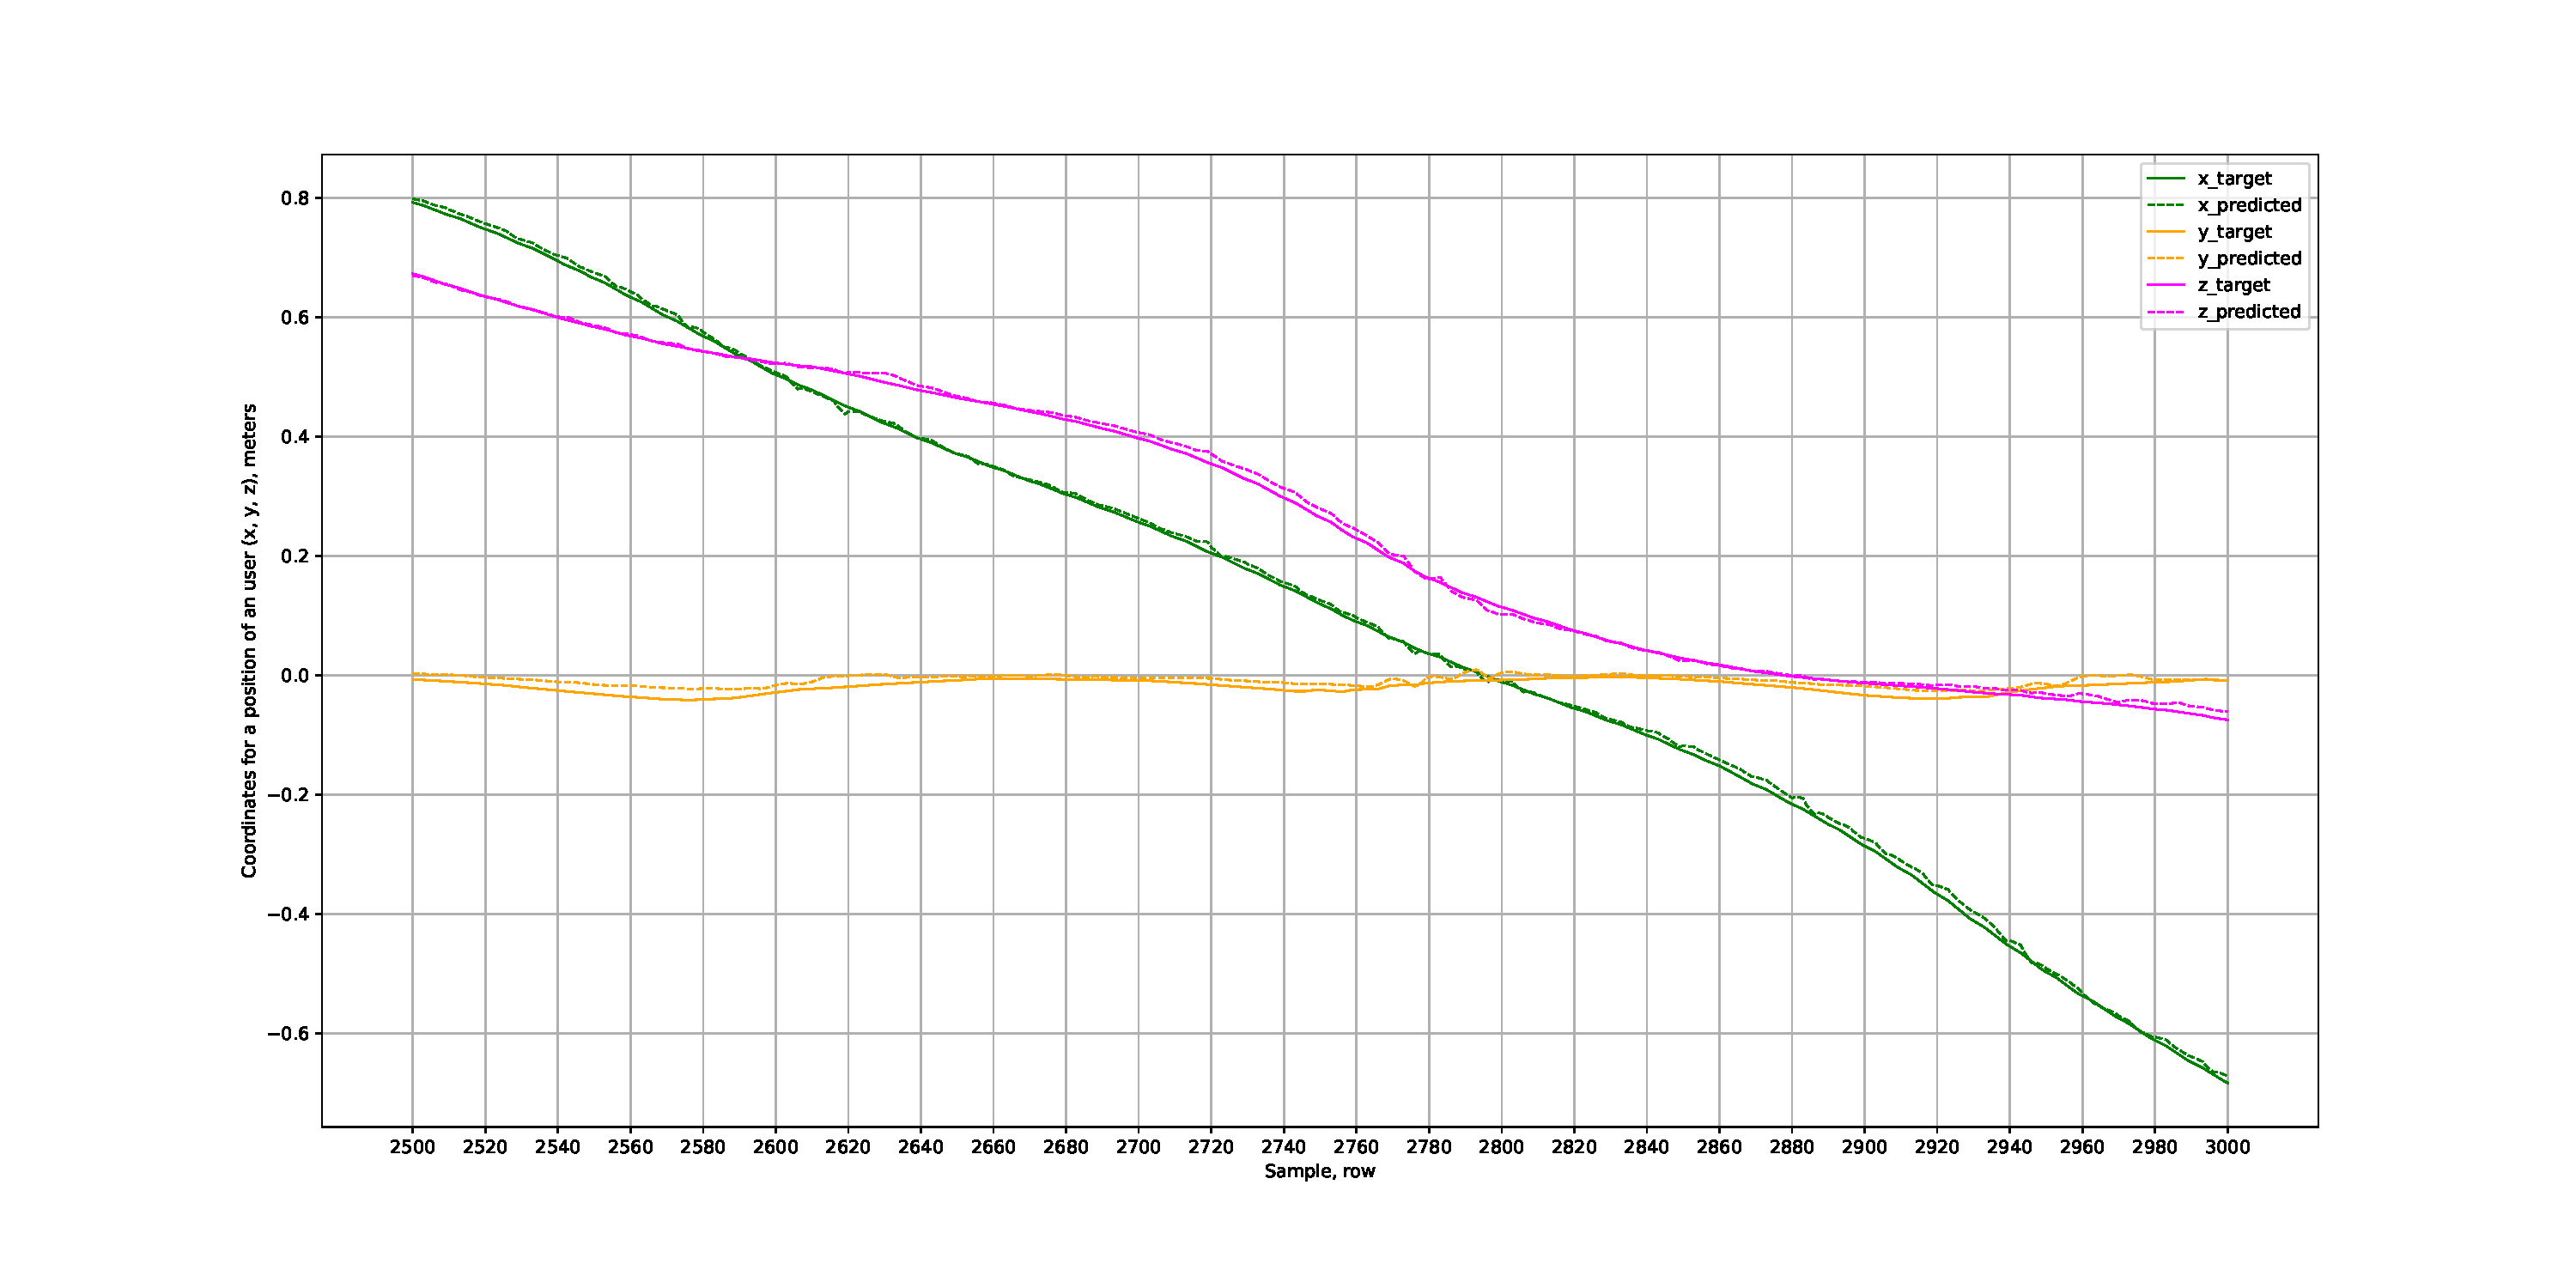
\includegraphics[width=0.9\textwidth, keepaspectratio]{gfx/lstm1_flipped-xyz_position.pdf}
		\caption{\label{fig:flip1} Outputs of LSTM1 model on dataset with flipped negative quaternions for x, y and z axes.}
	\end{center}
\end{figure}

\begin{figure}
	\begin{center}
		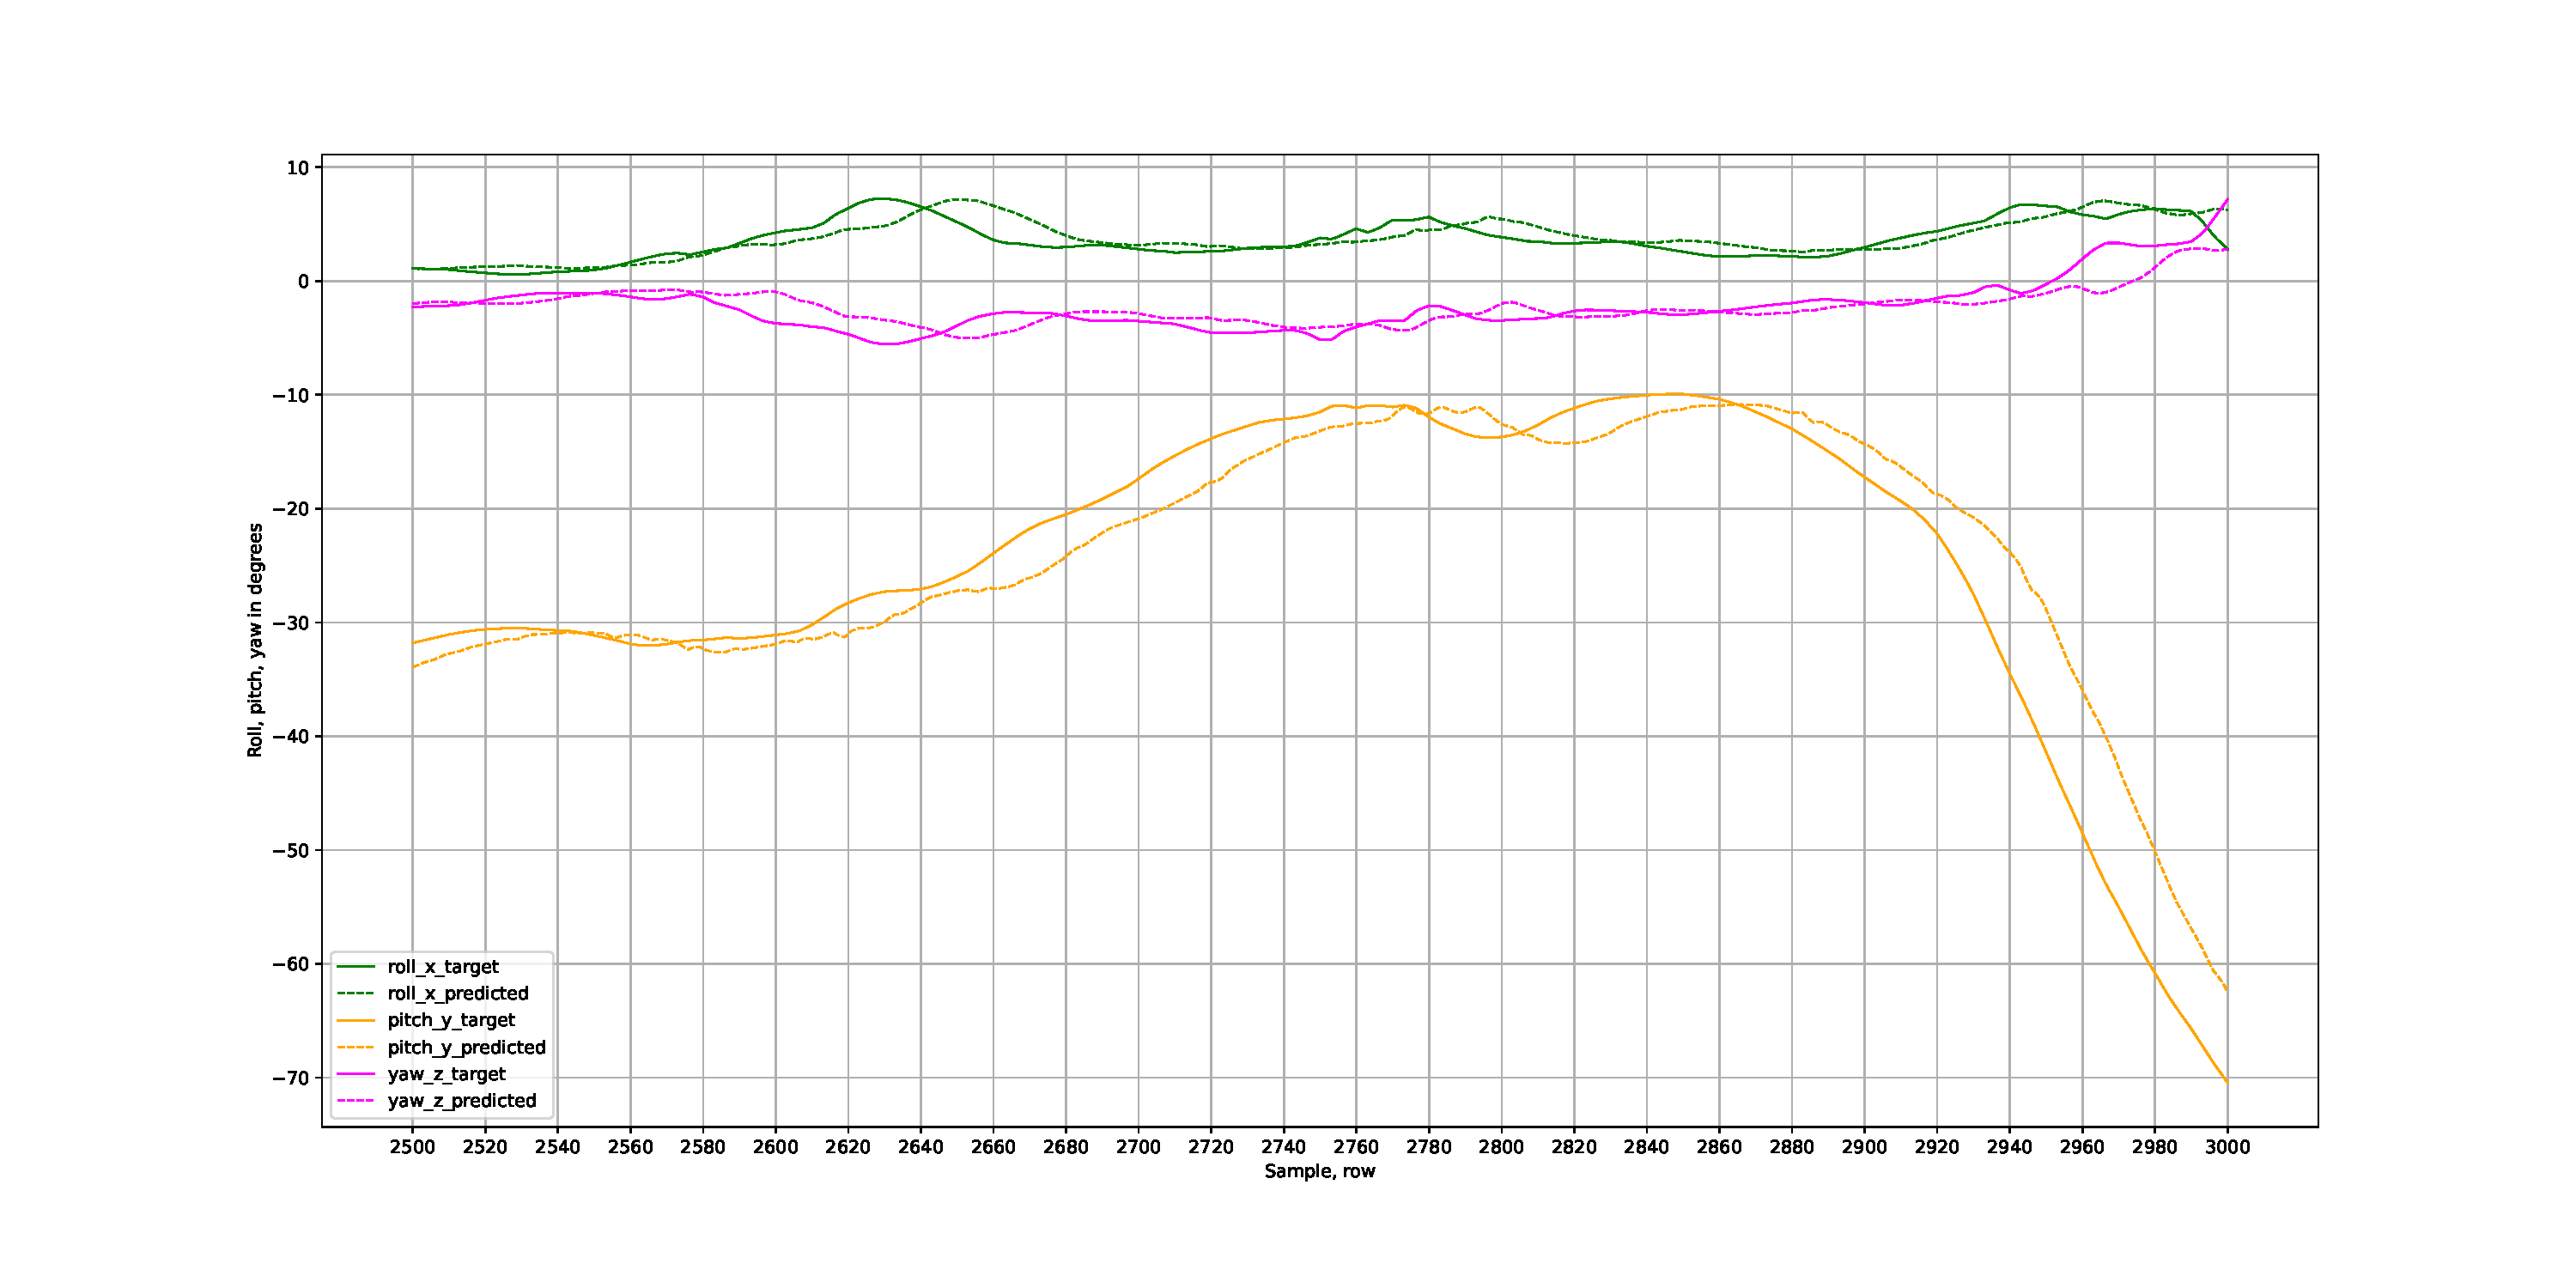
\includegraphics[width=0.9\textwidth, keepaspectratio]{gfx/lstm1_flipped-roll_pitch_yaw.pdf}
		\caption{\label{fig:flip2} Outputs of LSTM1 model on dataset with flipped negative quaternions for roll, pitch, yaw axes.}
	\end{center}
\end{figure}

Figures \ref{fig:interp1} and \ref{fig:interp2} show the predictions of the LSTM1 model on an interpolated dataset. The mean square error for the all three positional axes $MAE_{pos} = 0.019$m and root mean square error  $RMSE_{pos} = 0.028$m meaning the average distance between predicted position and the real position reduced from 7 cm to 2 cm if LSTM1 on interpolated dataset is used instead of Baseline. For all four quaternion components calculated metrics  are: $MAE_{rot} = 16.92^{\circ}$ and $RMSE_{rot}  =23.28^{\circ}$. LSTM1 predicts the rotation on an interpolated dataset worse than the Baseline model. The goal of the next experiment is to evaluate whether the flipping of negative quaternions can improve rotational prediction as it was expected on the preprocessing step.

Figures \ref{fig:flip1} and \ref{fig:flip2} show the predictions of the LSTM1 model on a dataset with flipped negative quaternions. The mean square error for the all three positional axes $MAE_{pos} = 0.013$m and root mean square error  $RMSE_{pos} = 0.015$m meaning the average distance between predicted position and the real position reduced from 7 cm to approx. 1.3 cm if LSTM1 on dataset with flipped negative quaternions is used instead of Baseline. For all four quaternion components calculated metrics are: $MAE_{rot} = 13.49^{\circ}$ and $RMSE_{rot}  =18.47^{\circ}$. Thus LSTM1 predicts the rotation on an flipped dataset slightly better than the Baseline model and there is also an improvement compared to prediction with interpolated dataset. Next experiments aim to evaluate whether the normalisation of positional data and dataset division can improve evaluation metrics. 

For the sake of place saving the plots of the rest datasets will not be added in the thesis. The division of dataset on pure positional dataset and pure rotational does not improve the prediction error. For positional dataset $MAE_{pos}$ increased to $0.078$m and root mean square error jumped to to $0.091$m what means that $MAE_{pos}$ error increased by $116.41\%$ and $RMSE_{pos}$ by $133,82\%$ compared to a Baseline. Surprisingly, opposed to the last experiment, in rotational dataset $MAE_{rot}$ decreased to $11.81^{\circ}$m and root mean square error reduced to $16.64^{\circ}$. It seems that for a prediction of the rotation the positional data can be eliminated from a dataset. The most interesting experiment done with a normalized dataset, Only position $(x, y, z)$ was scaled in range [0..1]. The $MAE_{pos}$ is slightly lower than Baseline's and is equal to $0.056$. This value must be considered as bad prediction because the better results are obtained with two previous datasets. Additionally, $RMSE_{pos}$ increased significantly to $0.197$ what is by $289\%$ worse than a Baseline prediction. However, it is surprising that rotational $MAE_{rot}$ decreased to $9.87^{\circ}$m and $RMSE_{rot}$ reduced to  $12.72^{\circ}$. 

For the LSTM1 model the best prediction is done for a future position using interpolated dataset with flipped negative quaternions and for rotation using a dataset with normalised position. The analysis of this phenomena is done in section \ref{sec:conclusion:analysis}.

\subsubsection{Batch size}
\label{sec:eval:experiments:early:batch}
A significant impact on the performance e.g. the prediction accuracy has a batch size used in LSTM or GRU models. The batch-size helps to learn the common patterns as important features by providing a fixed number of samples at one time. So that the model thus can distinguish the common features by looking at all the introduced samples of the batch. In most cases, an optimal batch size is set to 64. When this batch size was initially used with the LSTM model, it gave significant high MSE, RMSE, train and validation errors. Based on the performance observation during experiments with LSTM parameters, batch size fine-tuning was done. The experiments done by \textit{Aykut et al} in their works \cite{delay_compensation_360} and \cite{telepresence} proved that appropriate batch size can be found in range $2^{9}$ - $2^{11}$ (512 - 2048). Notice that a power of 2 is used as a batch size. The overall idea is to fit a batch of samples entirely in the CPU/GPU. Since, all the CPU/GPU comes with a storage capacity in power of two, it is advised to keep a batch size a power of two. Using a number different from a power of 2 could lead to poor performance. Experimentally is proved in this thesis that similar to works \cite{delay_compensation_360, telepresence}  batch size of $2^{8}$ - $2^{10}$ (256, 512 and sometimes 1024) produces the best prediction result on 6-DoF dataset if the other hyperparameters are set correctly. The smaller batch sizes (32, 64 and 128) resulted in the high values of evaluation metrics and it was obvious to notice during experiments the improving the metrics with increasing the batch size.

\subsubsection{Learning rate}
\label{sec:eval:experiments:early:lr}
Learning rate is a parameter of the extended version of stochastic gradient Adam optimizer. The learning rate determines how much an updating step influences the current value of the weights. 

If the learning rate is large then a correspondingly large modification of the weights $w_i$ happens on each epoch. In general, too large learning rate overshoots the local minimum in a cost function.

The small learning rate does not allow the model to neither successfully learn patterns in the data nor generalise them on the validation data. The prediction on the test data done by a model trained with a small value of learning rate results in significant high error. Fig. \ref{fig:lr} shows the training and validation loss of the 150 epochs of training with a learning rate of $1^{-6}$ that finished with $MAE = 3.70$. Models can neither learn on training data nor predict the new data on validation dataset. 
\begin{figure}[htb]
	\begin{center}
		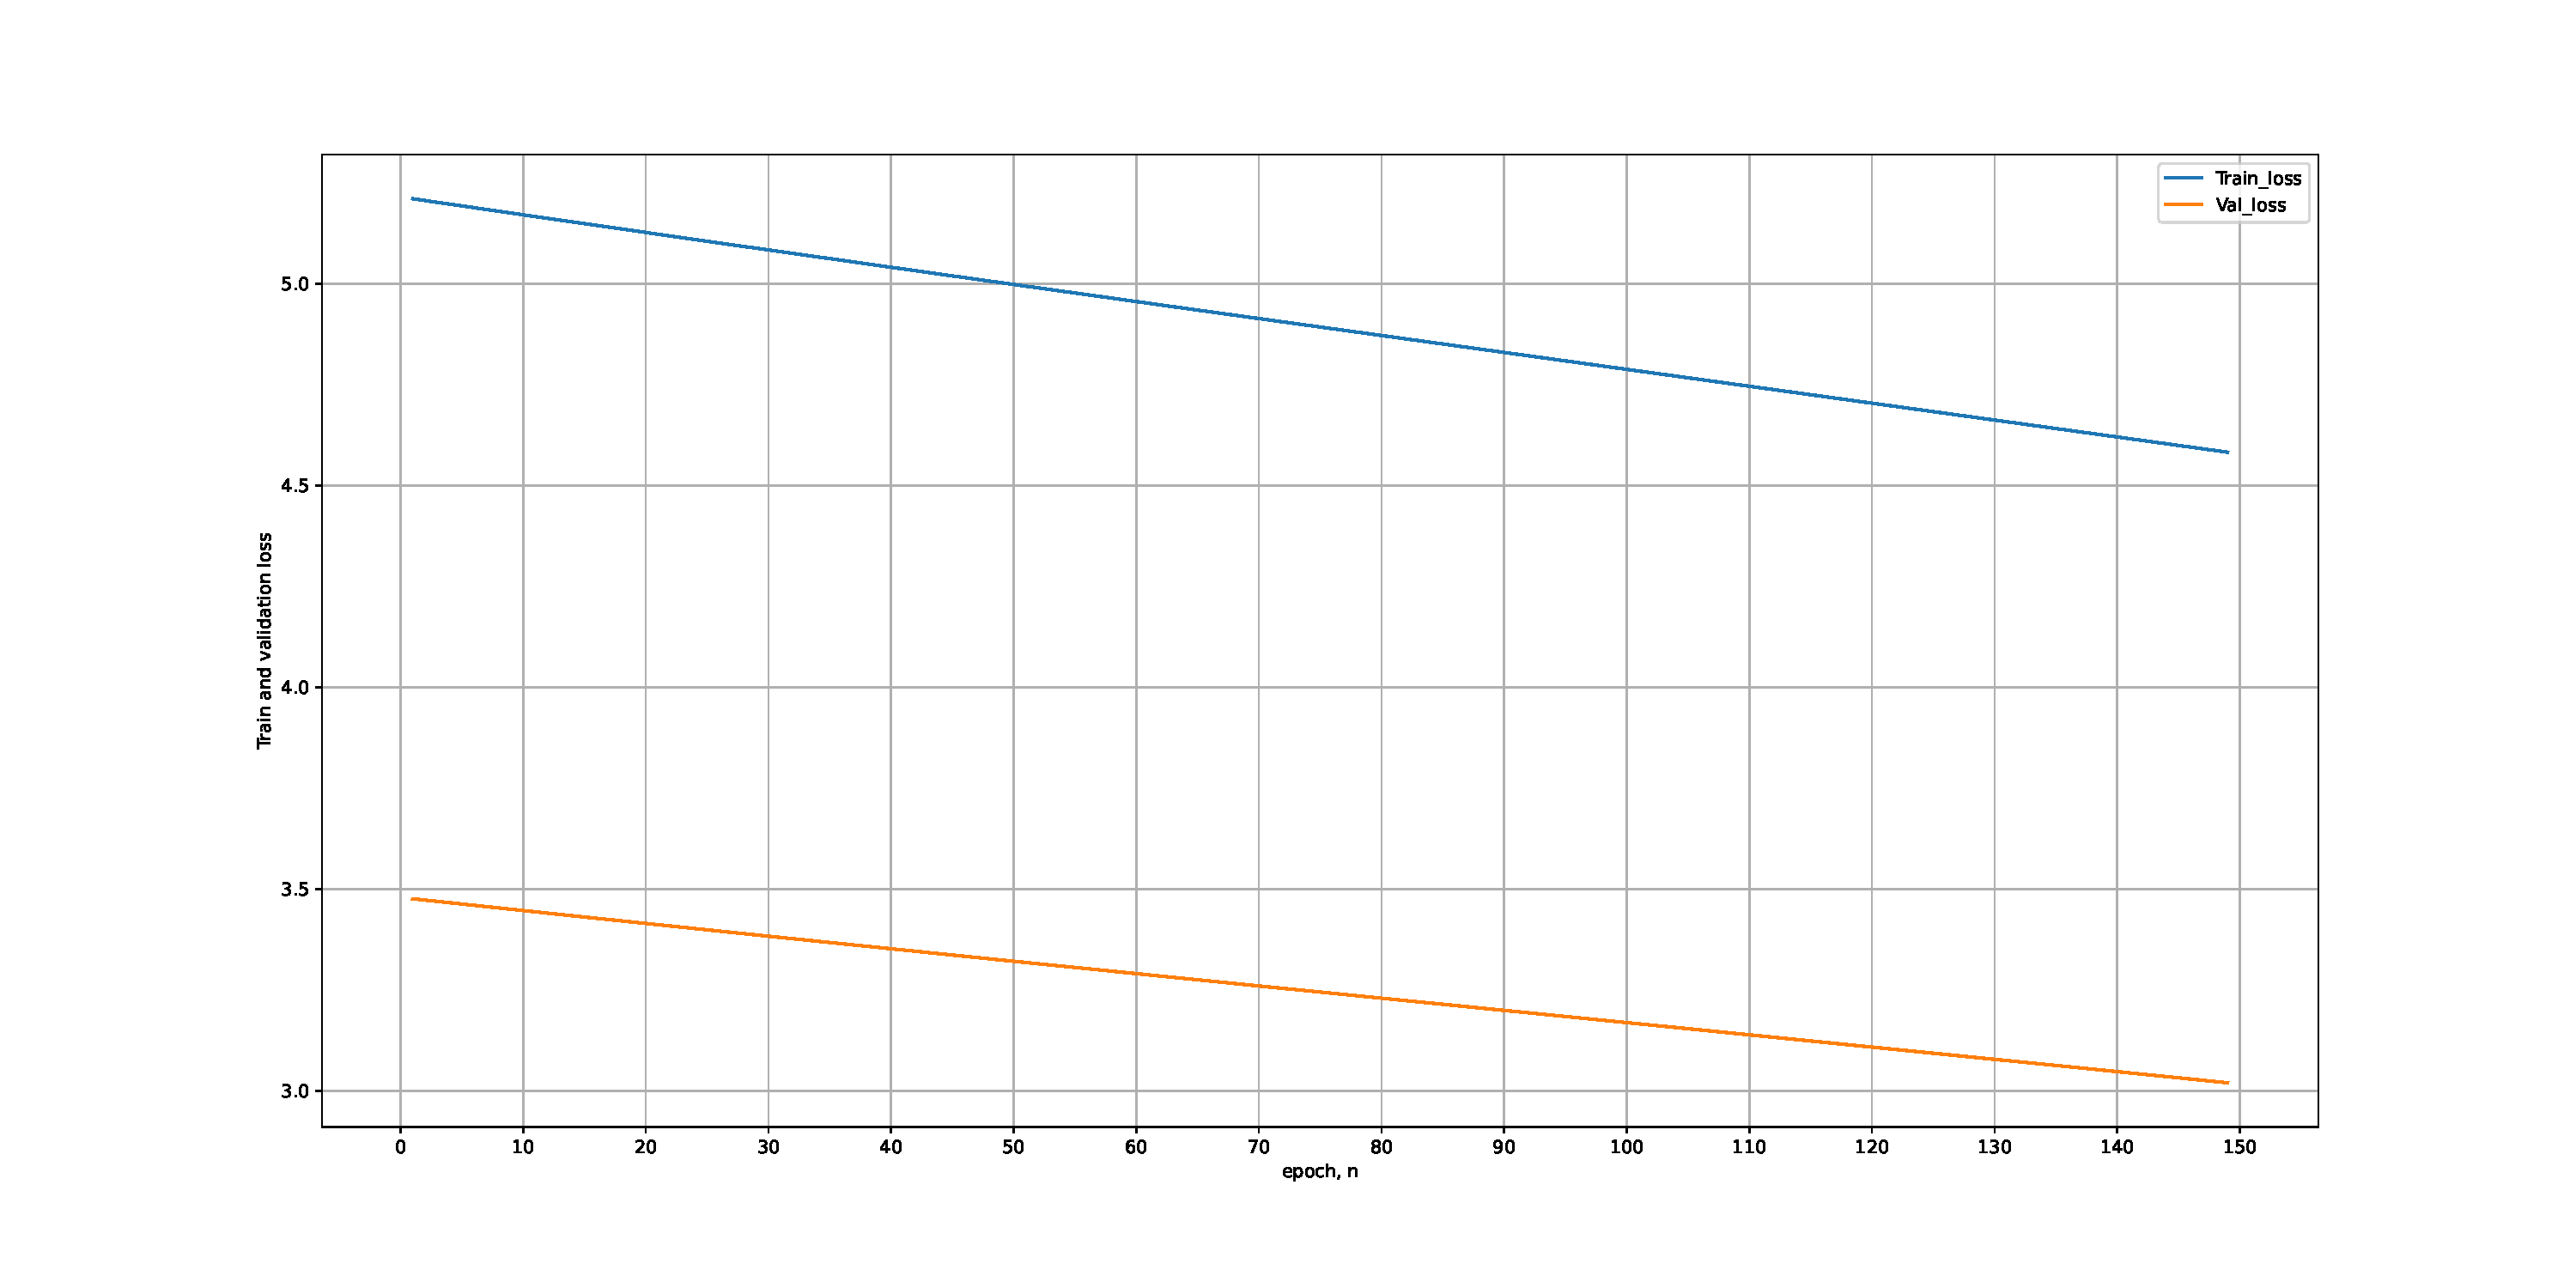
\includegraphics[width=1\textwidth, keepaspectratio]{gfx/lstm1_lr_low.pdf}
		\caption{\label{fig:lr} Plot of training and validation loss with small learning rate of Adam optimizer.}
	\end{center}
\end{figure}

In works \cite{delay_compensation_360, telepresence} by \textit{Aykut et al} the adaptively reducing learning rate is used. So that in the master thesis a learning rate decay scheduler was used to decrease the initial learning rate of $0.001$ every $50$ epochs by $50\%$. The values for learning rate, the amount of epochs to keep the value the same and the multiplier were found during experiments with grid parameters search. 

\subsubsection{Weight decay}
Adam optimizer has an additional term in the weight update rule that causes the weights to exponentially decay to zero, if no other update is scheduled. With weight decay after each update, the weights are multiplied by a factor less than 1. This prevents the weights from growing too large, and can be seen as gradient descent on a quadratic regularisation term. Thus weight decay is a regularisation technique used to avoid over-fitting. Indeed experiments showed that relatively large weight decay equal to $1^{-4} .. 1^{-8}$ make it possible for a model to overtrain so that training loss permanently decreases but validation loss fluctuates on the high level. Model can not generalise the learned pattern and predict successfully future values on never seen before data. 
\begin{figure}[htb]
	\begin{center}
		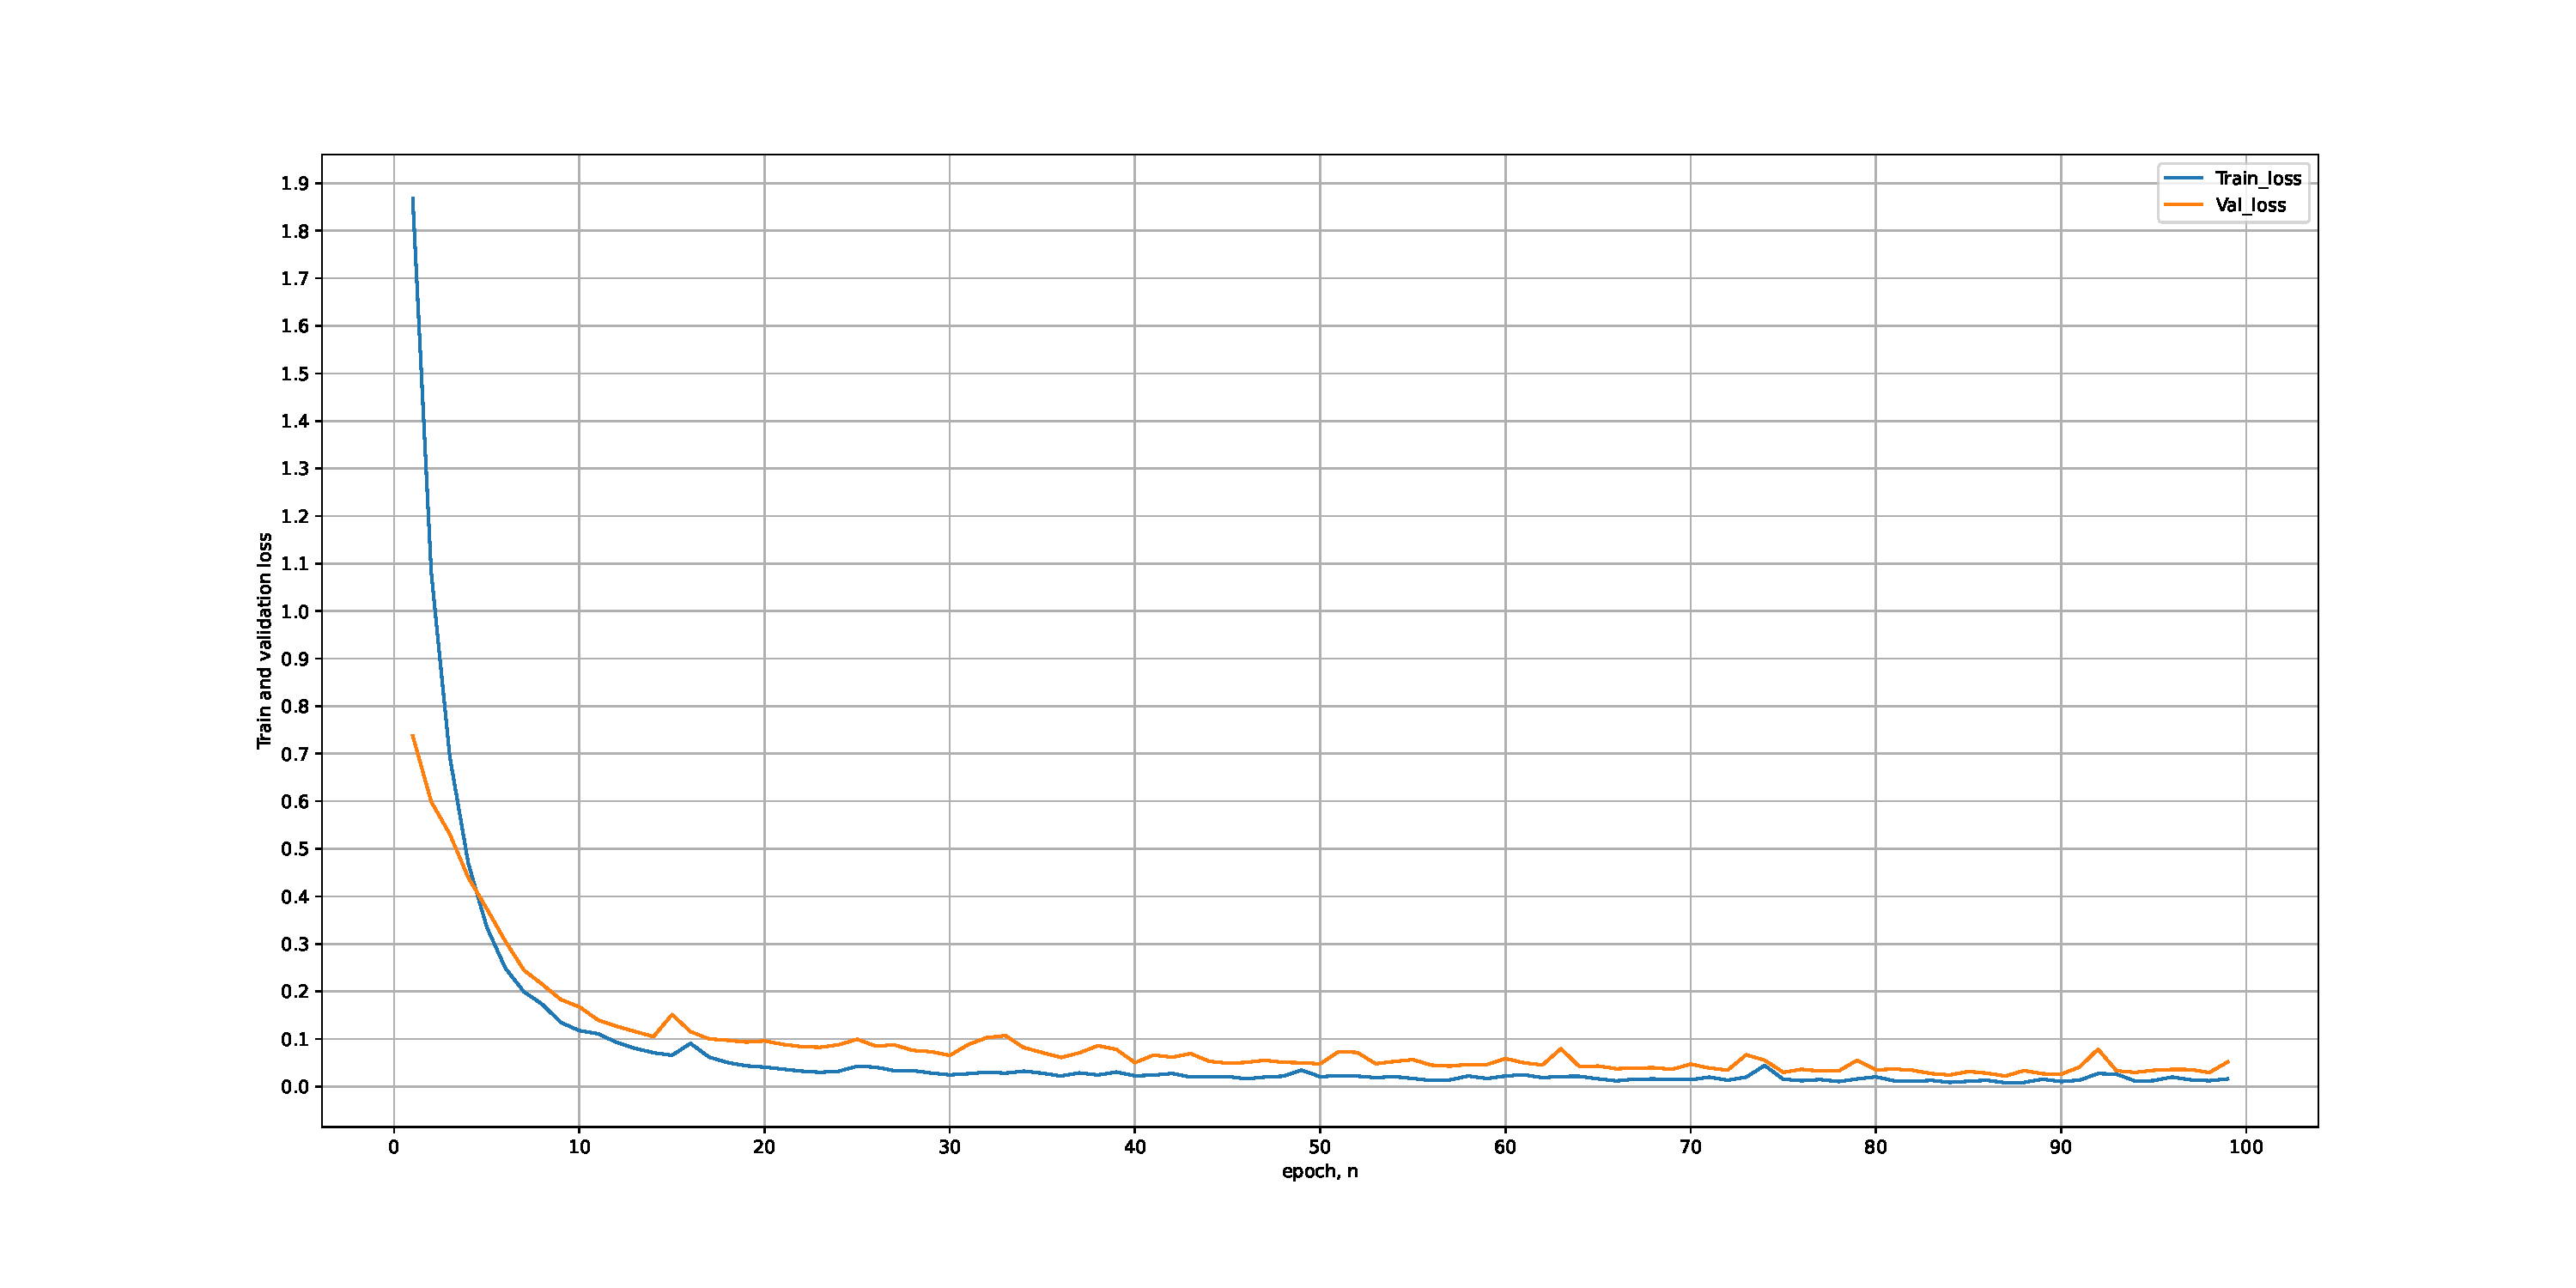
\includegraphics[width=1\textwidth, keepaspectratio]{gfx/lstm1_weight_decay_high.pdf}
		\caption{\label{fig:wd} Plot of training and validation loss with large weigh decay of Adam optimizer.}
	\end{center}
\end{figure}

Fig. \ref{fig:wd} illustrates both training and validation loss with large weight decay set to $1^{-6}$ of Adam optimizer. For the illustrative goal to avoid an elimination of the feeling of distance difference due to scale and to emphasise it, plot shows only 100 first epochs. It is seen that validation loss remains on high lever and starts to increase.  

Best values for weight decay parameter of Adam optimizer set to  $1^{-12}$ for LSTM and GRU model after parameter grid search on GPU cluster.

\subsection{Prediction with LSTM}
\label{sec:eval:experiments:lstm}
This section presents the results of best prediction using LSTM models and also shows the predictions with LSTM variants that are considered to fail either to predict better than Baseline or to be used as improvement compared to Baseline predictions. The role of different parameters such as batch size, learning rate and weight decay is described in section \ref{sec:eval:experiments:early}. The training and evaluation is this and next sections are done on an interpolated dataset with flipped negative quaternions. 

During preprocessing step Euler angles (yaw, pitch, roll) were calculated from quaternions and these parameters are used for visualisation purposes. The quaternions of the model's predictions are also converted to Euler angles so that $MAE$ and $RMSE$ units in degrees are similar to plotted information. 

The best prediction results with LSTM1 are already presented in figures \ref{fig:flip1} and \ref{fig:flip2} in the section above. Thereby LSTM1 model has best performance on interpolated dataset with flipped negative quaternions and all evaluation metrics were improved. $MAE_{pos} = 0.013$m, $RMSE_{pos} = 0.015$m, $MAE_{rot} = 13.49^{\circ}$ and $RMSE_{rot}  =18.47^{\circ}$. Compared to Baseline this means 80\% improvement of prediction for position and almost 10\% improvement for rotation. The average distance between predicted position and the real position reduced from 7 cm to circa 1.3 cm.
\begin{figure}[t]
	\begin{center}
		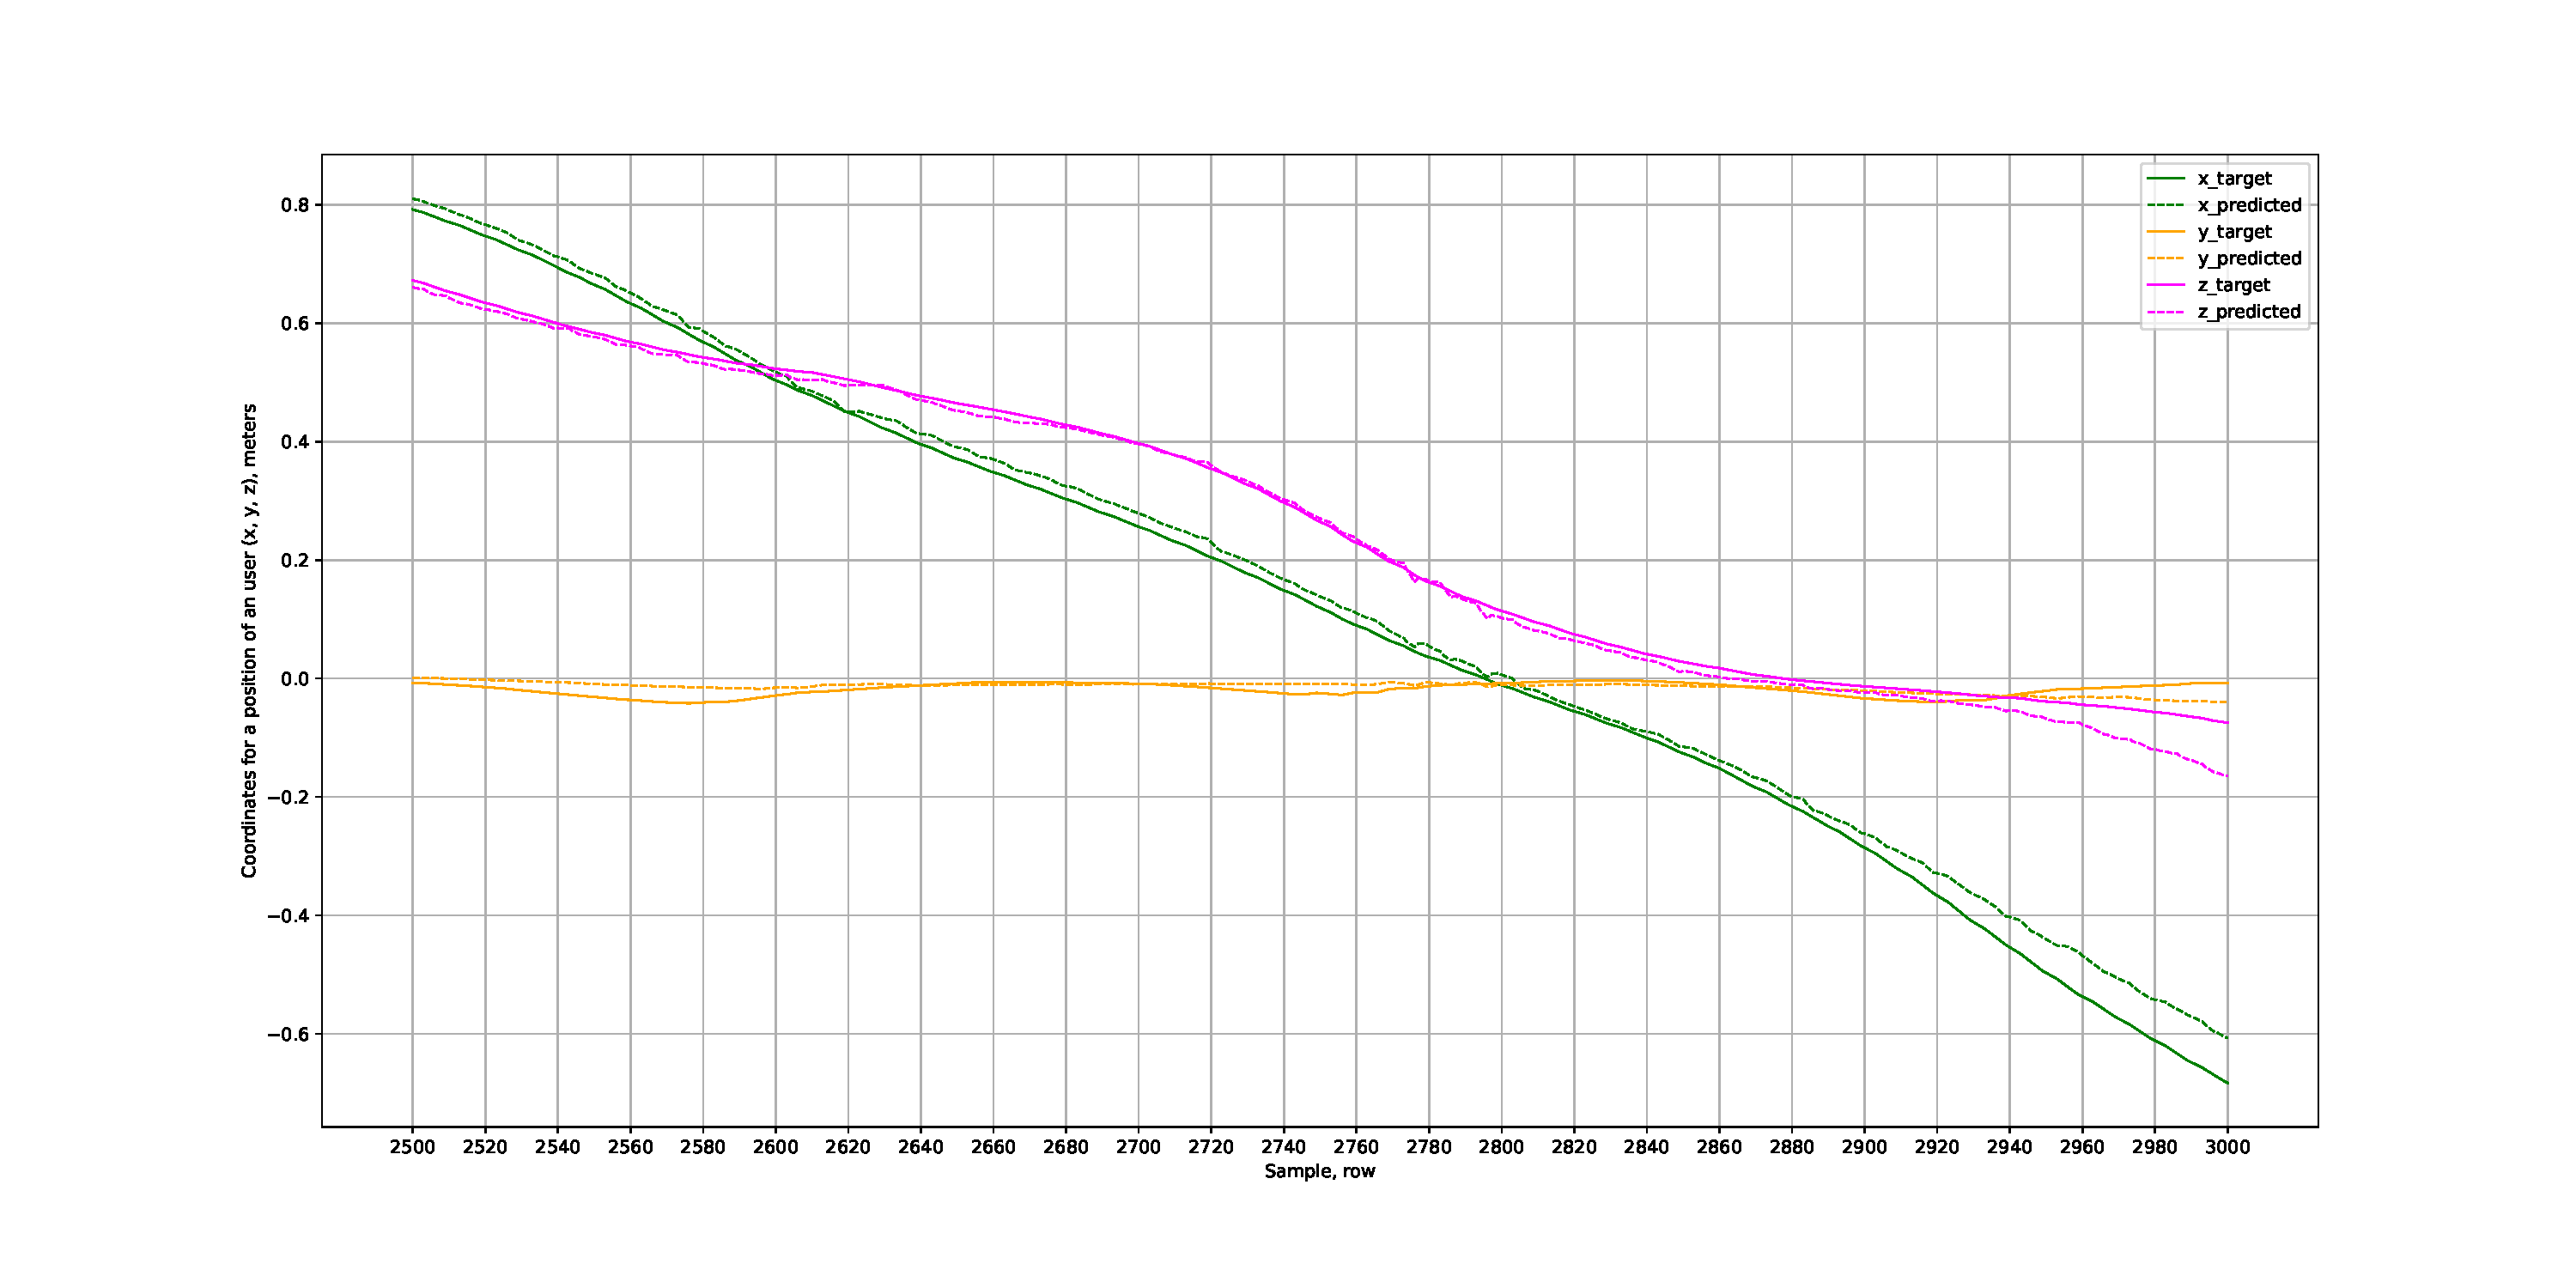
\includegraphics[width=0.9\textwidth, keepaspectratio]{gfx/lstm2_relu-xyz_position.pdf}
		\caption{\label{fig:lstm2-1} Outputs of LSTM2 model with ReLU activation function for x, y and z axes.}
	\end{center}
\end{figure}

\begin{figure}
	\begin{center}
		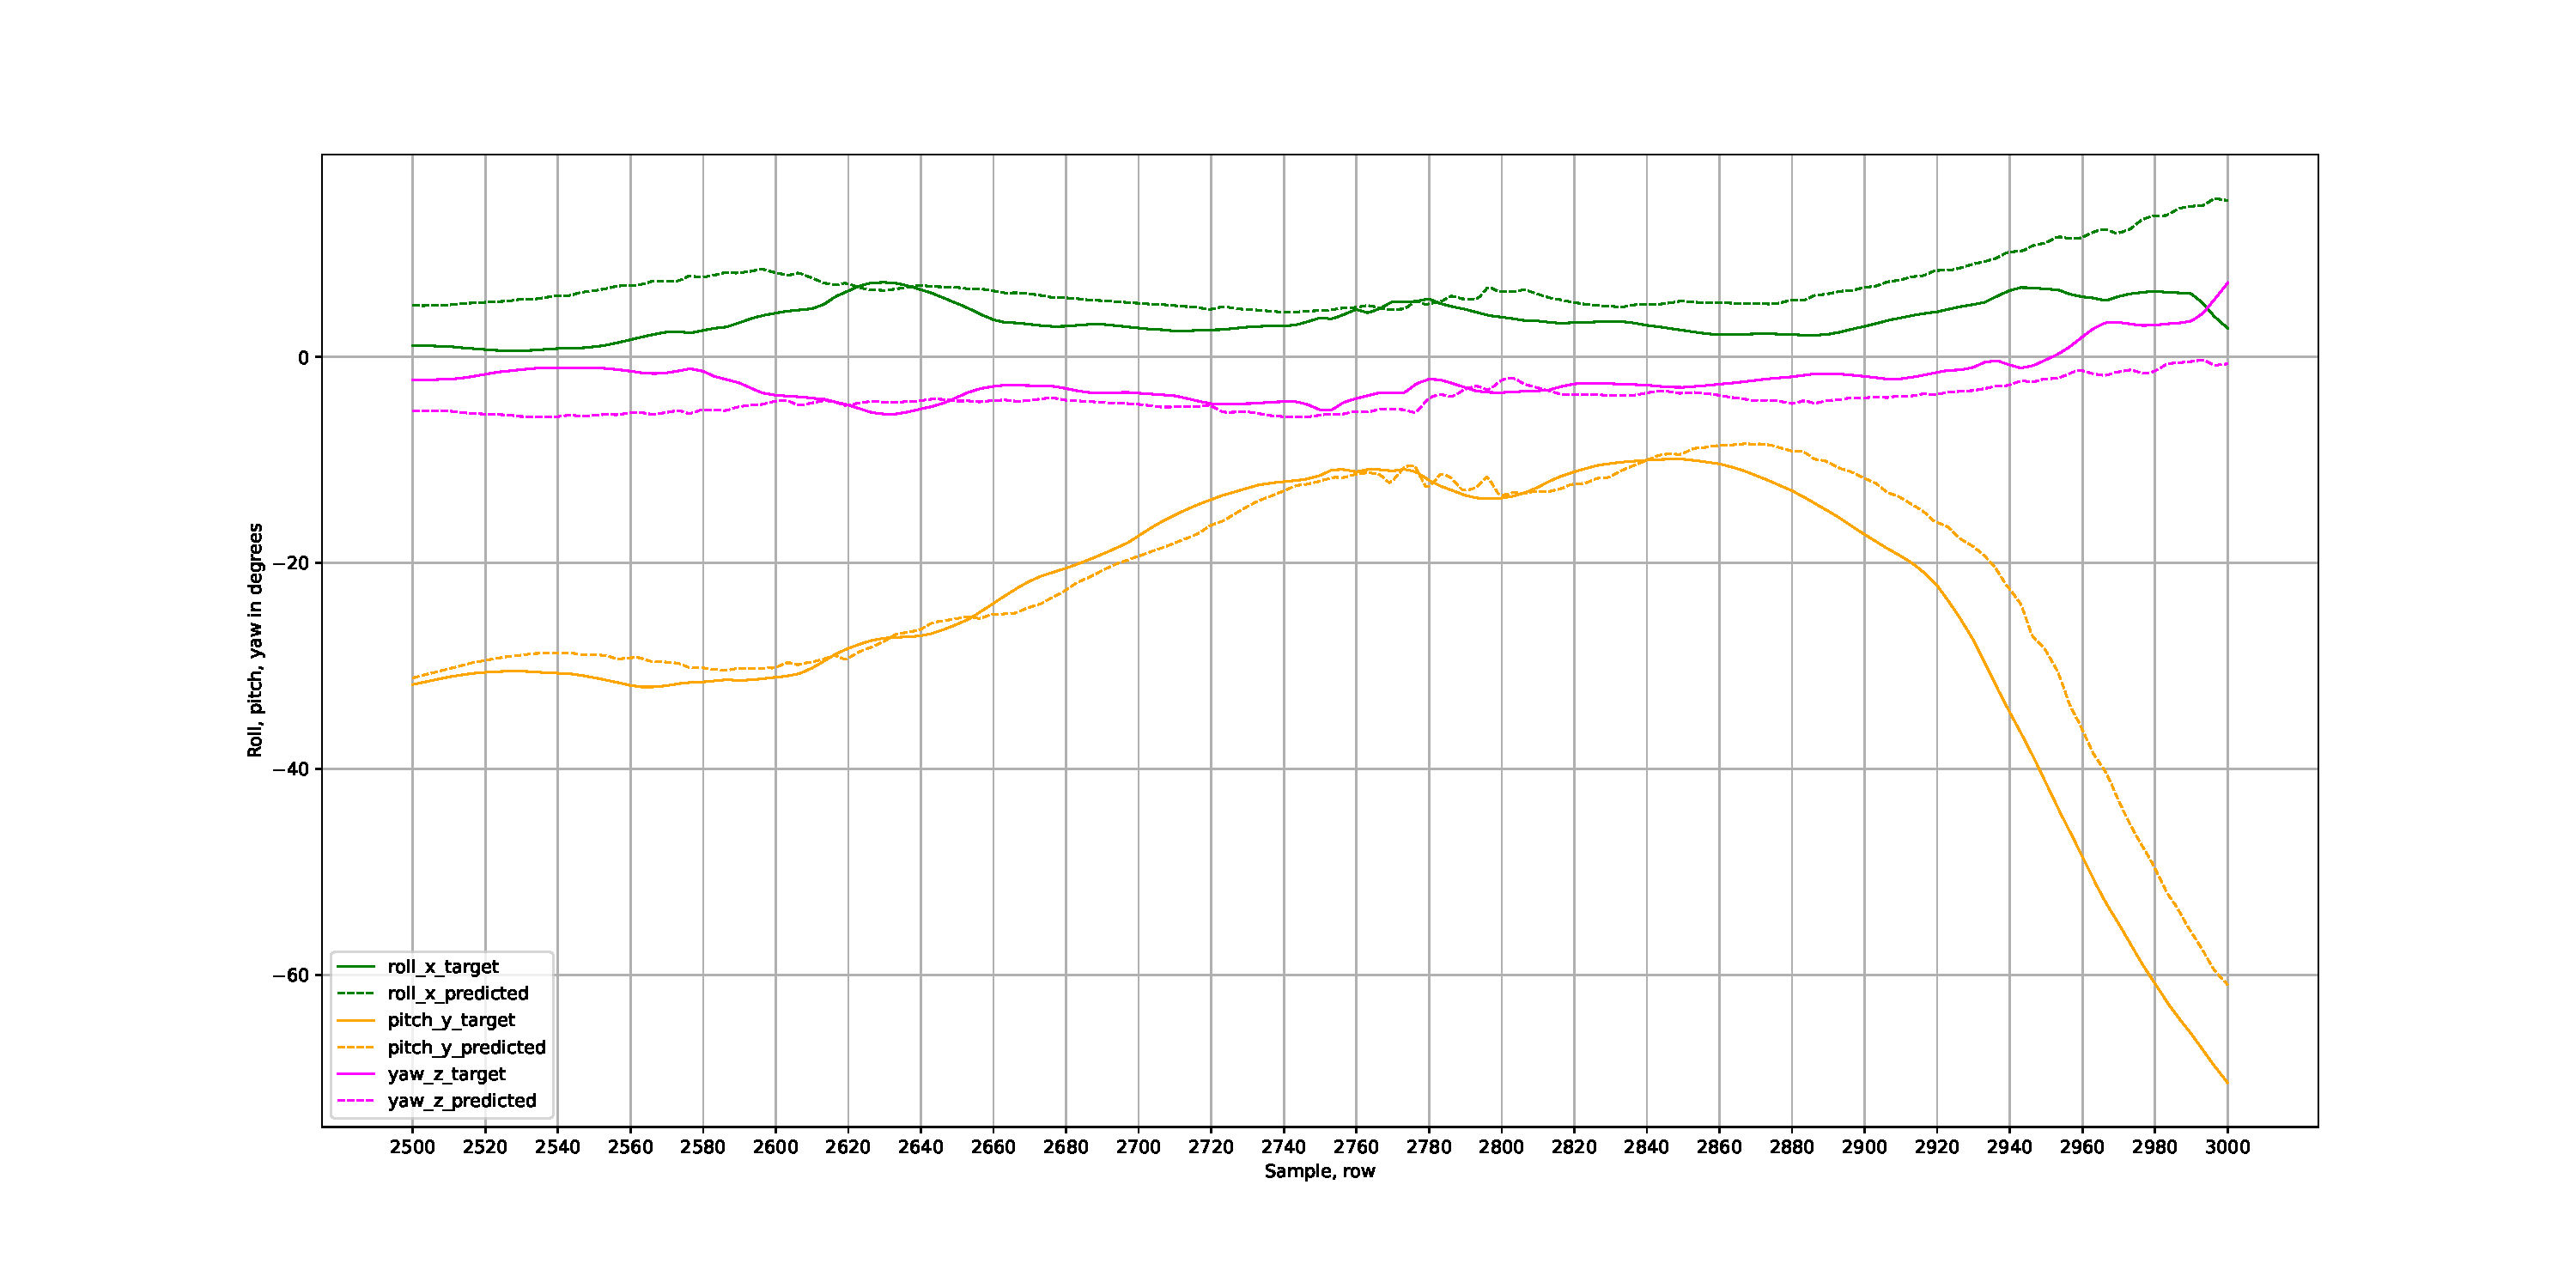
\includegraphics[width=0.9\textwidth, keepaspectratio]{gfx/lstm2_relu-roll_pitch_yaw.pdf}
		\caption{\label{fig:lstm2-2} Outputs of LSTM2 model with ReLU activation function for roll, pitch, yaw axes.}
	\end{center}
\end{figure}

Fig. \ref{fig:lstm2-1}, \ref{fig:lstm2-2} displays the same range of prediction outputs for the LSTM2 model with the $ReLU$ activation function. It was mentioned in section \ref{sec:impl:model:arch:lstm} that this architecture experimentally leads to higher evaluation errors compared to LSTM1 model. Indeed,  $MAE_{pos} = 0.055$m, $RMSE_{pos} = 0.185$m, $MAE_{rot} = 22.86^{\circ}$ and $RMSE_{rot}  =30.88^{\circ}$. In Fig. \ref{fig:lstm2-1} and \ref{fig:lstm2-2} it is clear to see that distance between predicted values and real values is larger compared to LSTM1 and is similar and somewhere worse than with the Baseline model. Thus graphs for $roll$ and $pitch$ have bigger gaps between real and predicted values. The predictions for $x$ and $z$ axes do not exactly follow the trend of the graph and real and predicted values have obvious distance between plotted graphs. 

\begin{figure}[t!]
	\begin{center}
		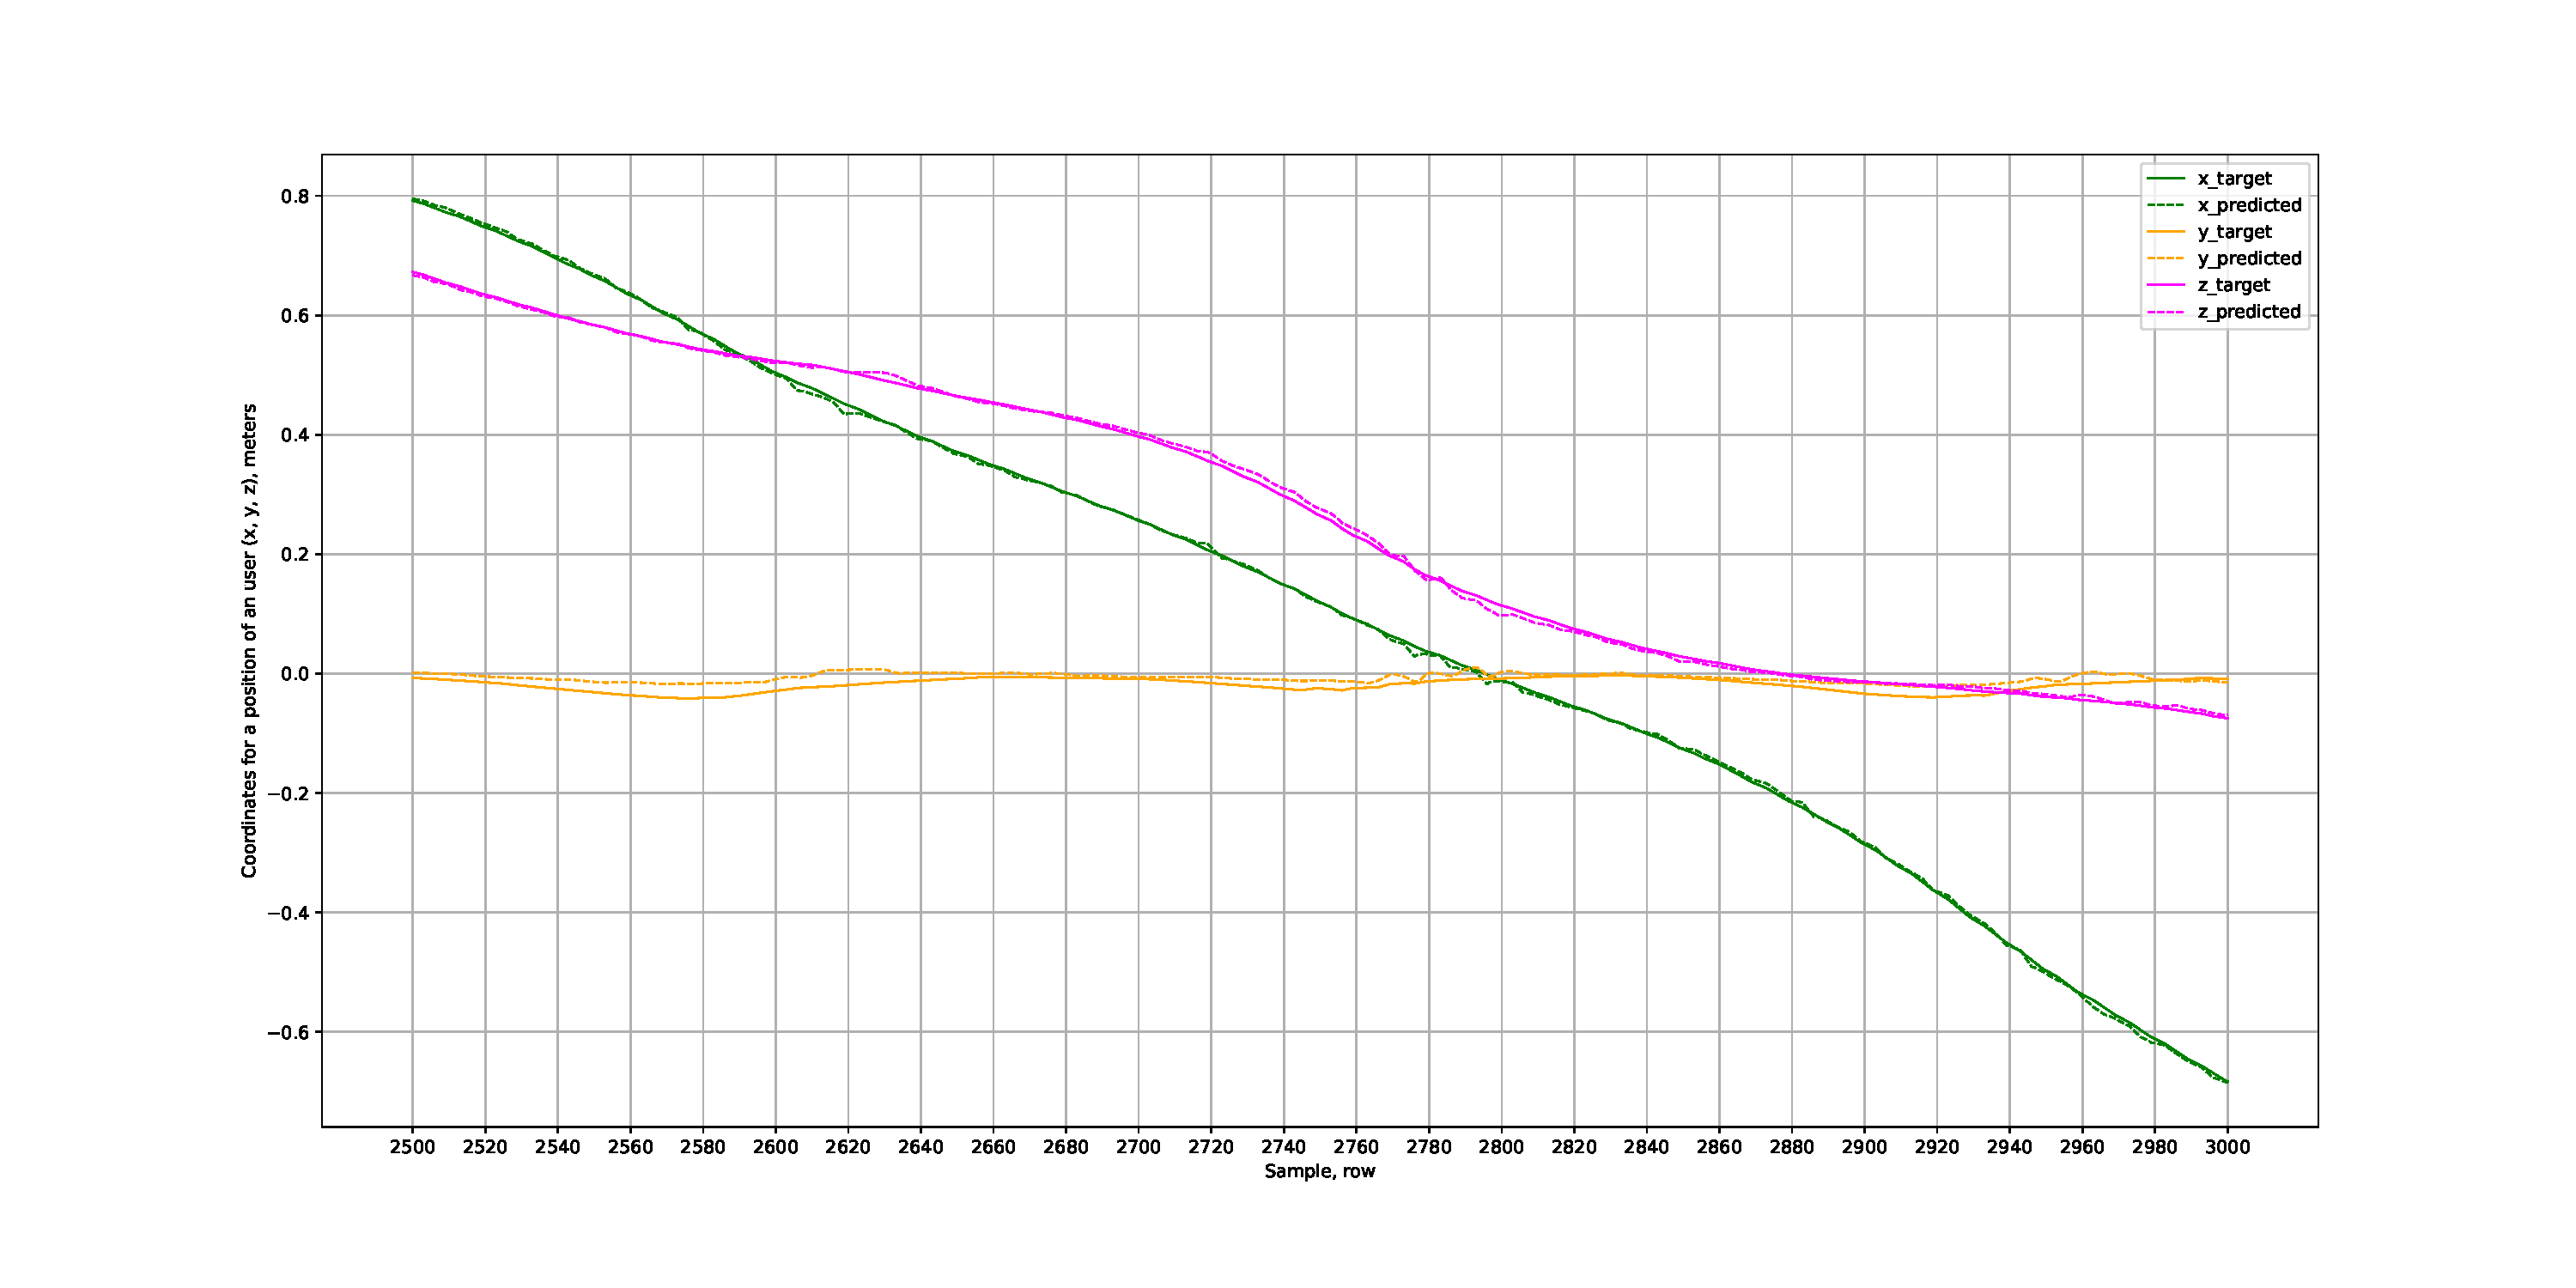
\includegraphics[width=0.9\textwidth, keepaspectratio]{gfx/lstm3_mish-xyz_position.pdf}
		\caption{\label{fig:lstm3-1} Outputs of LSTM3 model with Mish activation function for x, y and z axes.}
	\end{center}
\end{figure}

\begin{figure}[b!]
	\begin{center}
		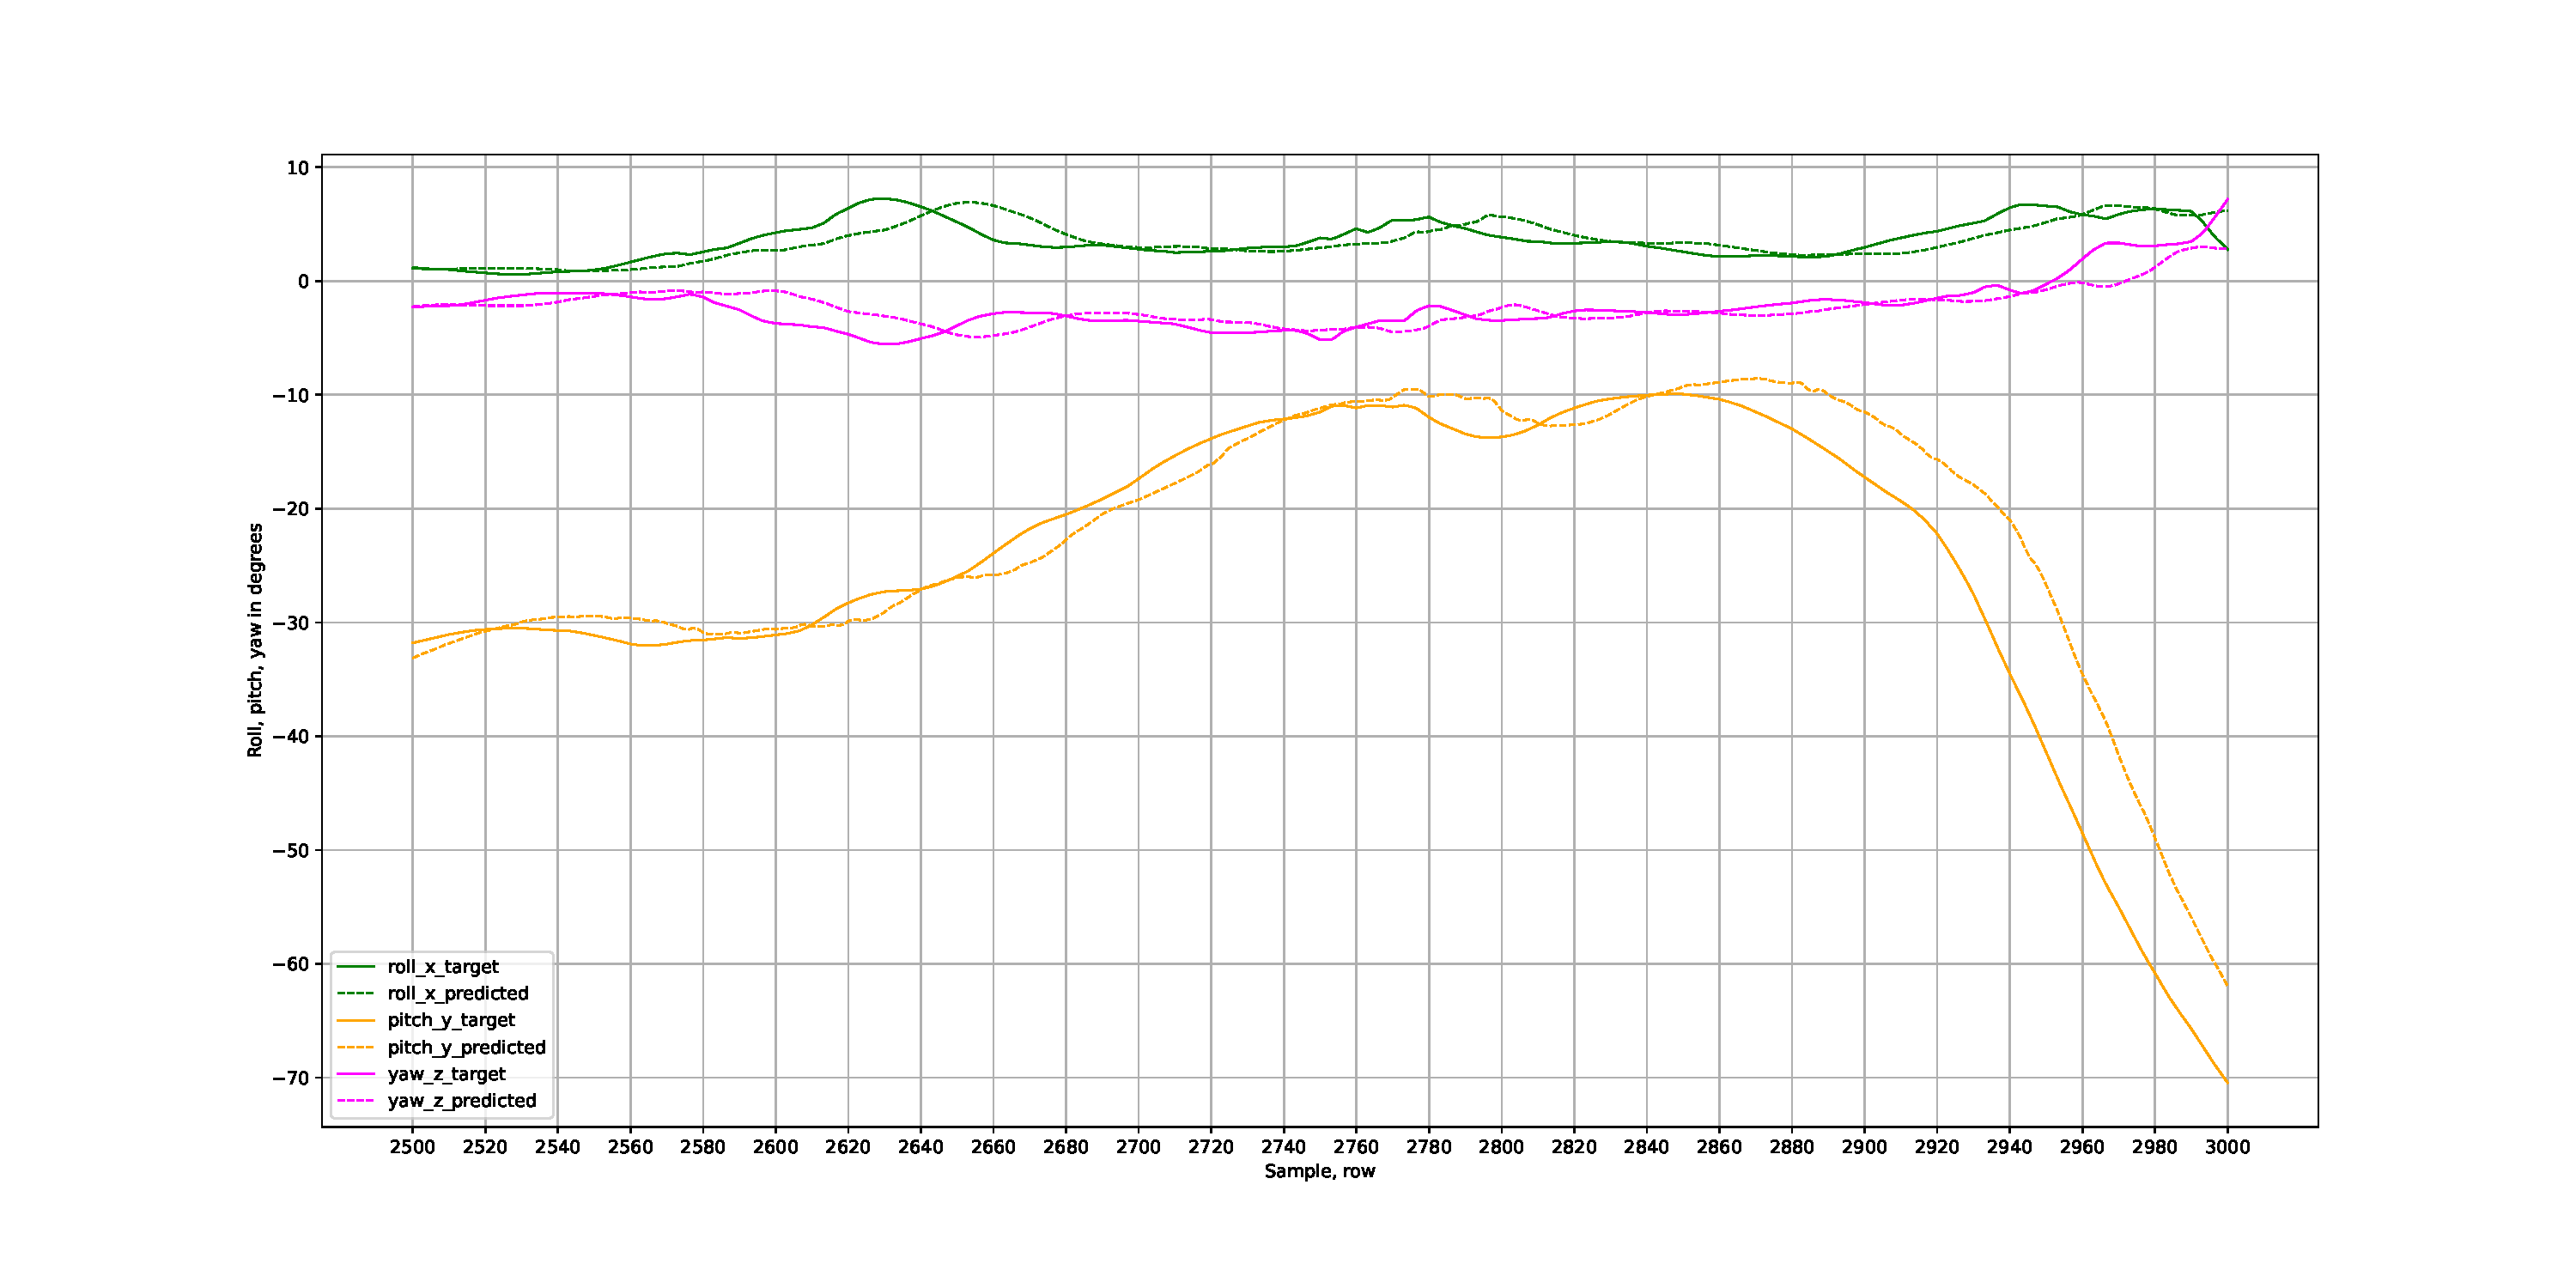
\includegraphics[width=0.9\textwidth, keepaspectratio]{gfx/lstm3_mish-roll_pitch_yaw.pdf}
		\caption{\label{fig:lstm3-2} Outputs of LSTM3 model with Mish activation function for roll, pitch, yaw axes.}
	\end{center}
\end{figure}

The same outputs for the LSTM3 model with $ReLU$ activation function are illustrated in Fig. \ref{fig:lstm3-1}, \ref{fig:lstm3-2}. This architecture experimentally can improve the evaluation metrics comparing both to LSTM1 and Baseline models. The best metrics are as follows:  $MAE_{pos} = 0.012$m, $RMSE_{pos} = 0.014$m, $MAE_{rot} = 13.18^{\circ}$ and $RMSE_{rot}  =17.28^{\circ}$.

In Fig. \ref{fig:lstm2-1} and \ref{fig:lstm2-2}  The predictions for $x$ and $z$ can almost exactly follow the trend of the graph (that was is smaller $MAE$ means graphically) and real and predicted values have almost no obvious big distance between plotted graphs. There are also slight improvements of $roll$ and $pitch$ predictions but the evaluation metrics are still not low enough to allow predictions to exactly repeat the graph of real values. 

A three-layered stacked LSTM4 model with introduced additional dropout added after all but last recurrent layer and Mish activation function has similar to LSTM2 positional error but the rotational error drastically increased to $MAE_{rot} = 42^{\circ}$ and $RMSE_{rot}  =48^{\circ}$. The more complex model not only requires significantly more time to train but also has problems optimising parameters in a way that can optimally fit the training instances. 

\subsection{Prediction with GRU}
\label{sec:eval:experiments:gru}
This section presents the best result achieved with a pure GRU model without additional activation functions with simple one-layered architecture. 

GRU1 is the best evaluated model. It results with the smallest positional and rotational error. The evaluation metrics are: $MAE_{pos} = 0.009$m, $RMSE_{pos} = 0.011$m, $MAE_{rot} = 8.68^{\circ}$ and $RMSE_{rot}  =12.29^{\circ}$. Compared to Baseline this means 87\% improvement of prediction for position and almost 40\% improvement for rotation. The average distance between predicted position and the real position is reduced from 7 cm and GRU1 average error is less than 1 cm.  
\begin{figure}[b!]
	\begin{center}
		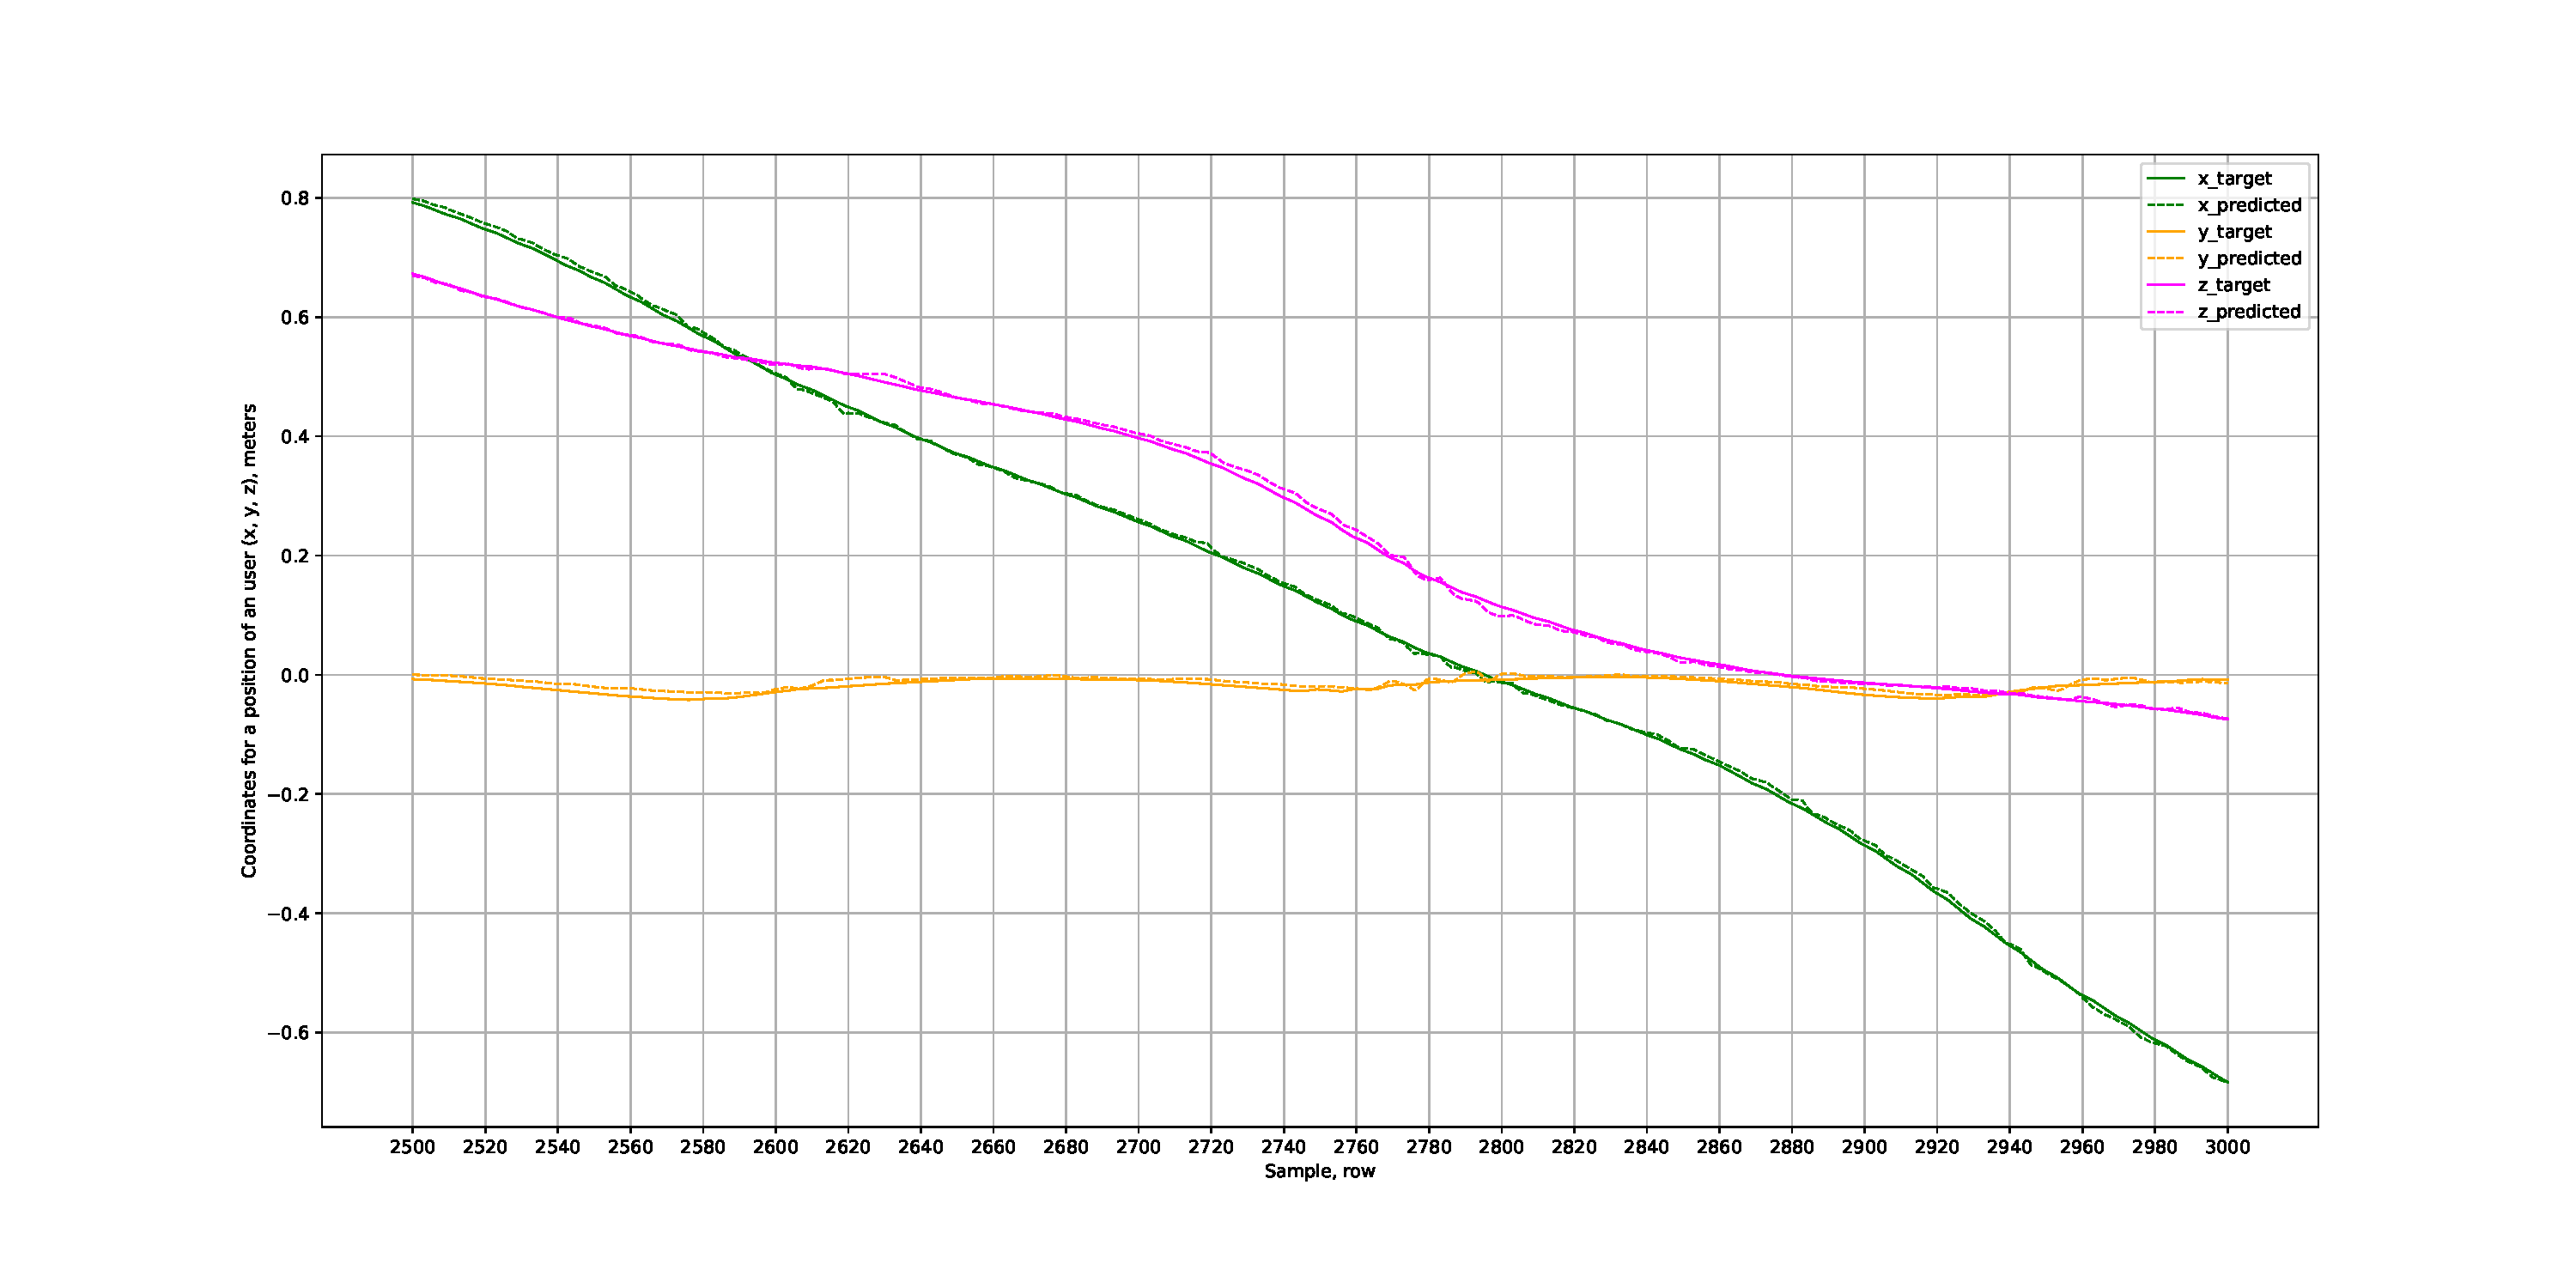
\includegraphics[width=0.8\textwidth, keepaspectratio]{gfx/gru1-xyz_position.pdf}
		\caption{GRU1 outputs for position (x, y, z) for rows 5000..5500.}
		\label{fig:gru1-1}
	\end{center}
\end{figure}

GRU1 results for rotation prediction on the full interpolated dataset with flipped negative quaternions outperformed the results of experiment done with a dataset containing only rotational data. Recall, in that experiment $MAE_{rot}$ decreased to $11.81^{\circ}$m and root mean square error reduced to  $16.64^{\circ}$ comparing to predictions done by the same model on the dataset containing position and rotation.
\begin{figure}[t!]
	\begin{center}
		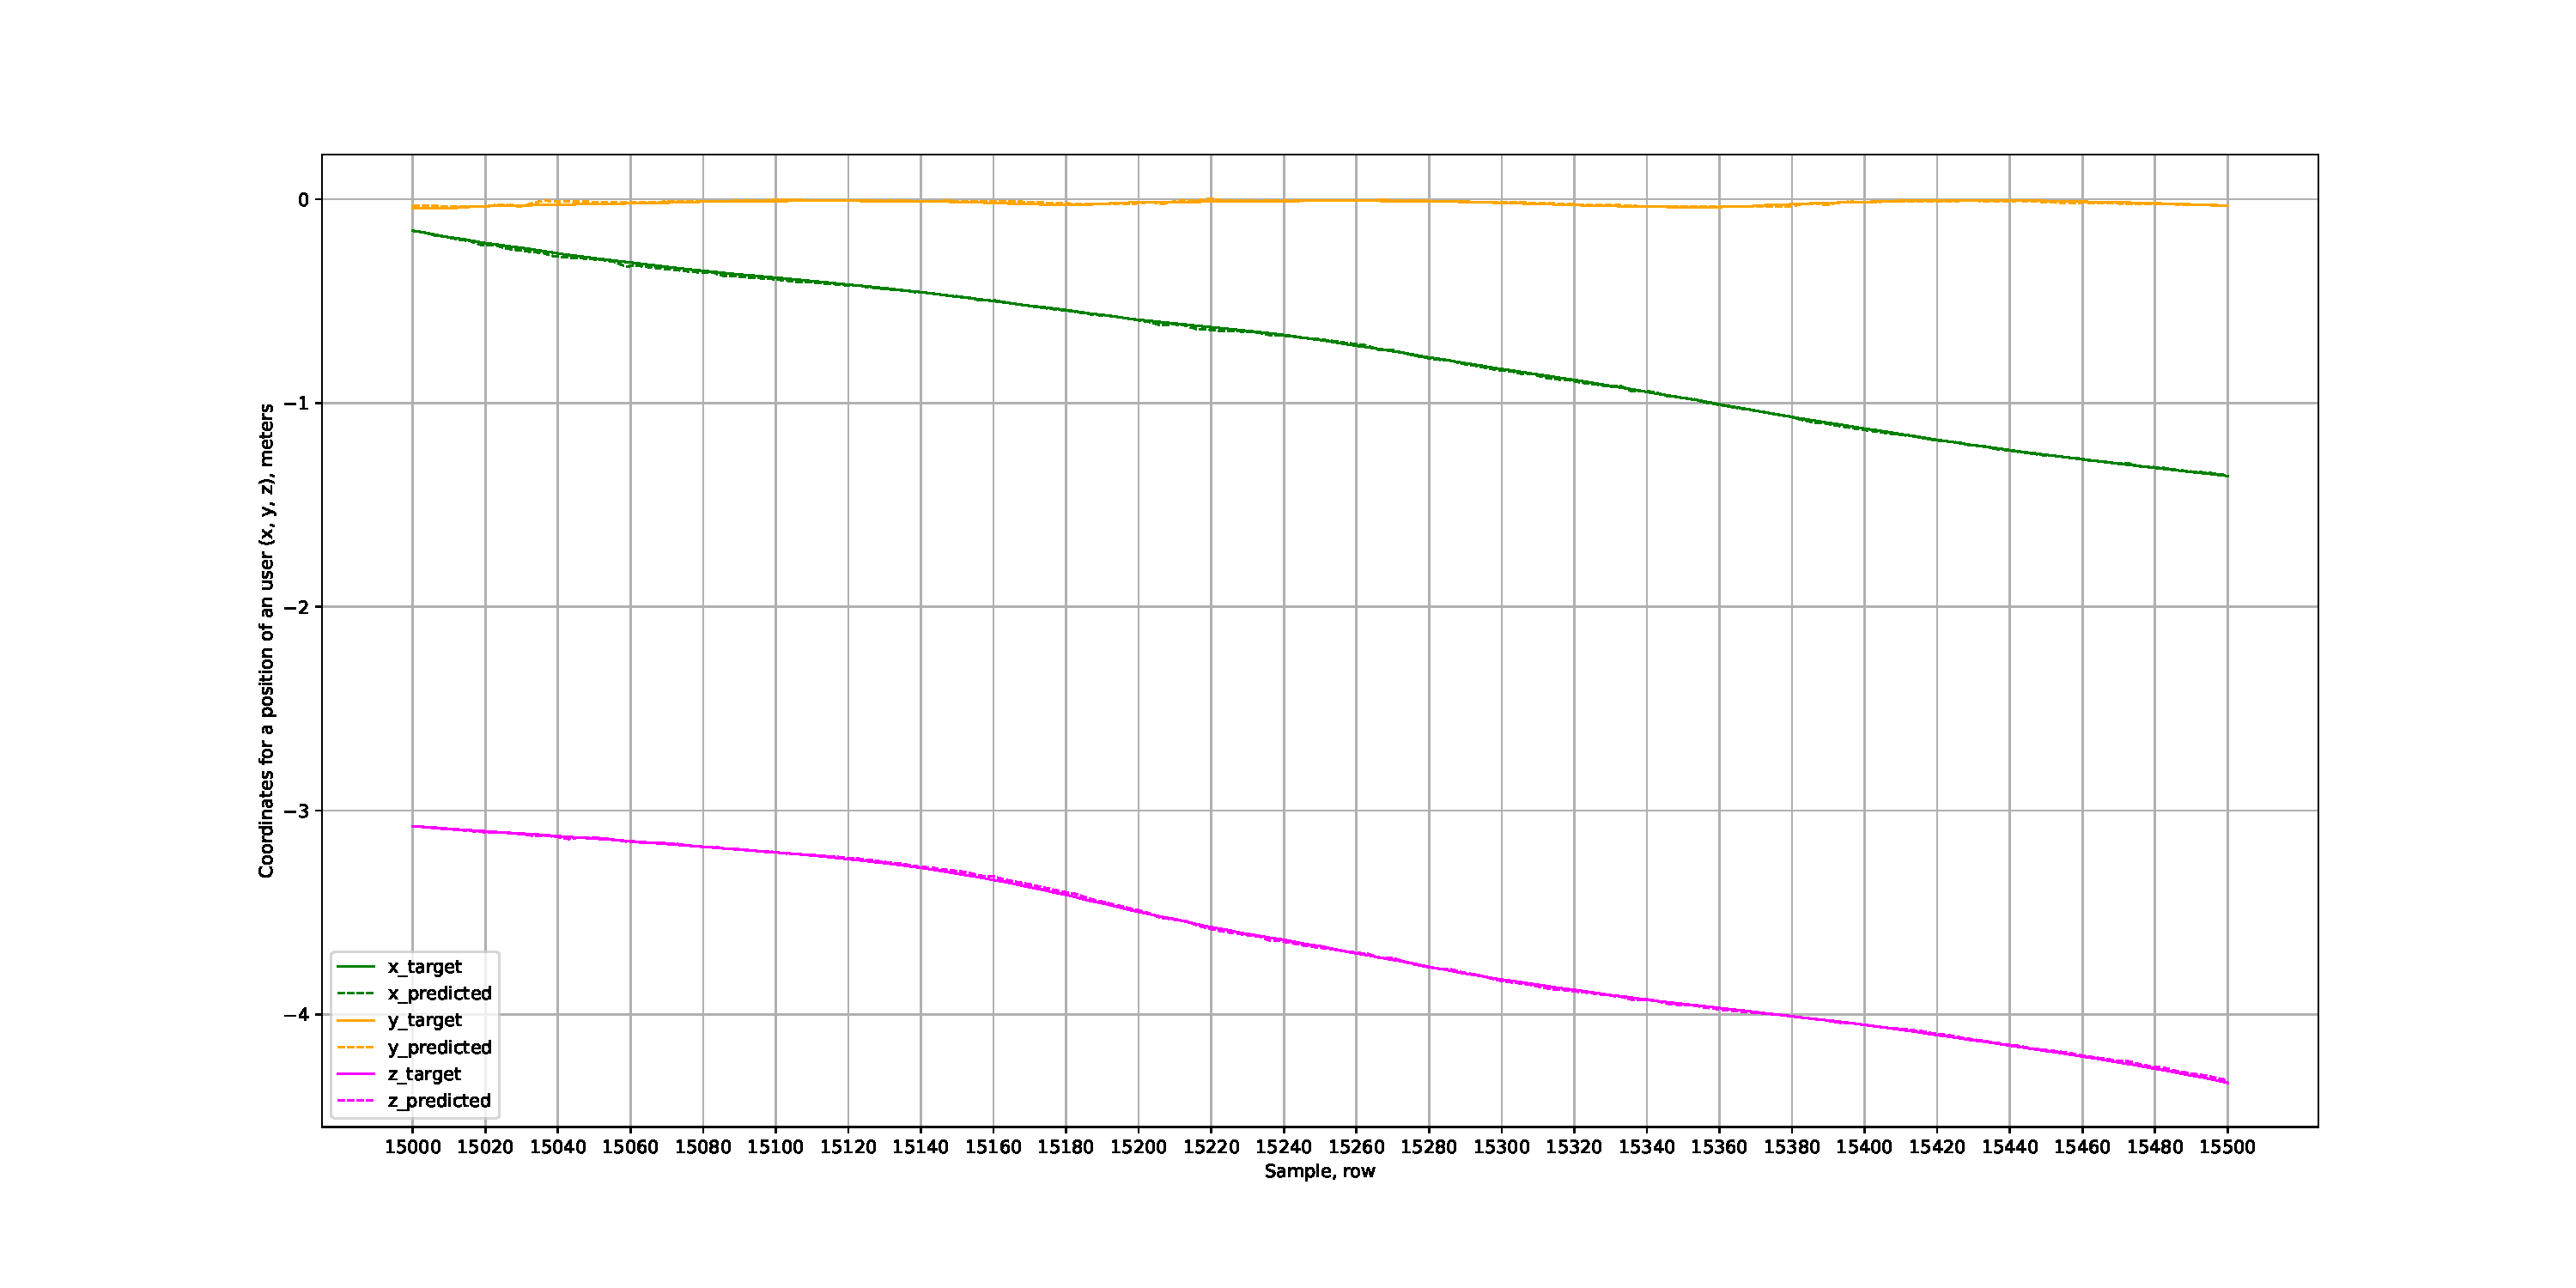
\includegraphics[width=0.8\textwidth]{gfx/gru1-xyz_position_15000.pdf}
		\caption{GRU1 outputs for position (x, y, z) for rows 15000..15500.}
		\label{fig:gru1-2}
	\end{center}
\end{figure}

Figures \ref{fig:gru1-1},  \ref{fig:gru1-2} and \ref{fig:gru1-3} plot predicted values over real for position data $(x, y, z)$. The range took so that first it is the same 500 samples near to the beginning of the dataset as used for visualisation with previous models. Additionally to emphasise accuracy the 500 samples in the middle of the dataset are taken and the same amount of samples is chosen near the end of the dataset. 
\begin{figure}[t!]
	\begin{center}
		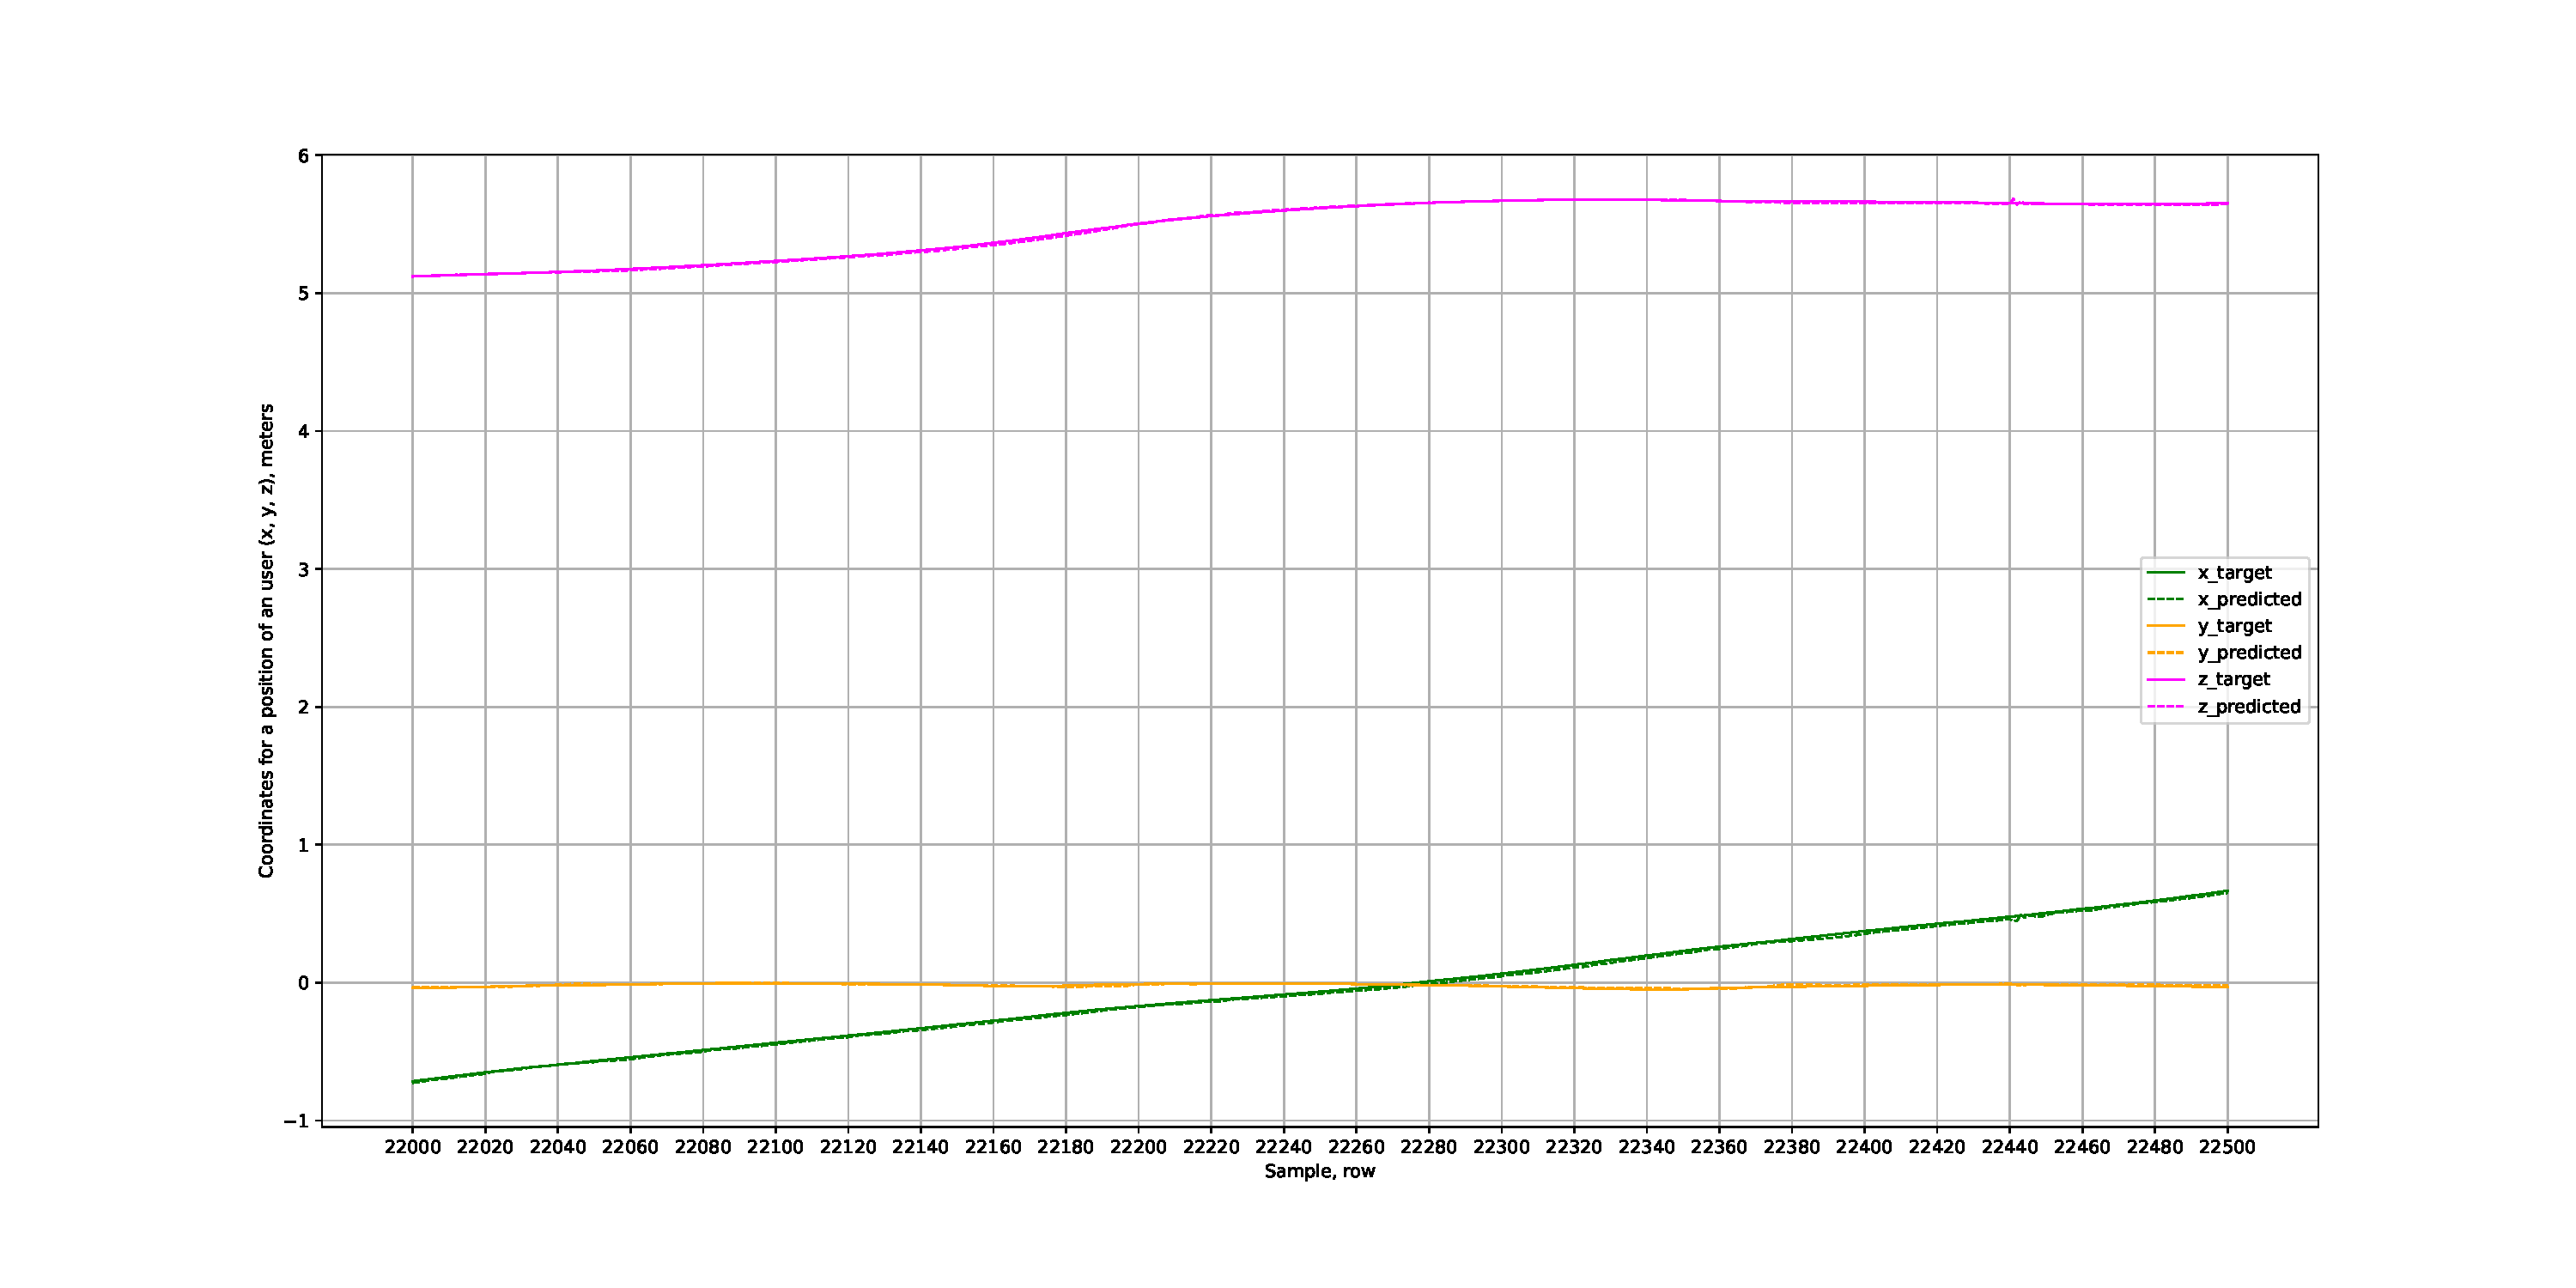
\includegraphics[width=0.8\textwidth, keepaspectratio]{gfx/gru1-xyz_position_21000.pdf}
		\caption{GRU1 outputs for position (x, y, z) for rows 22000..22500.}
		\label{fig:gru1-3}
	\end{center}
\end{figure}
\begin{figure}[t!]
	\begin{center}
		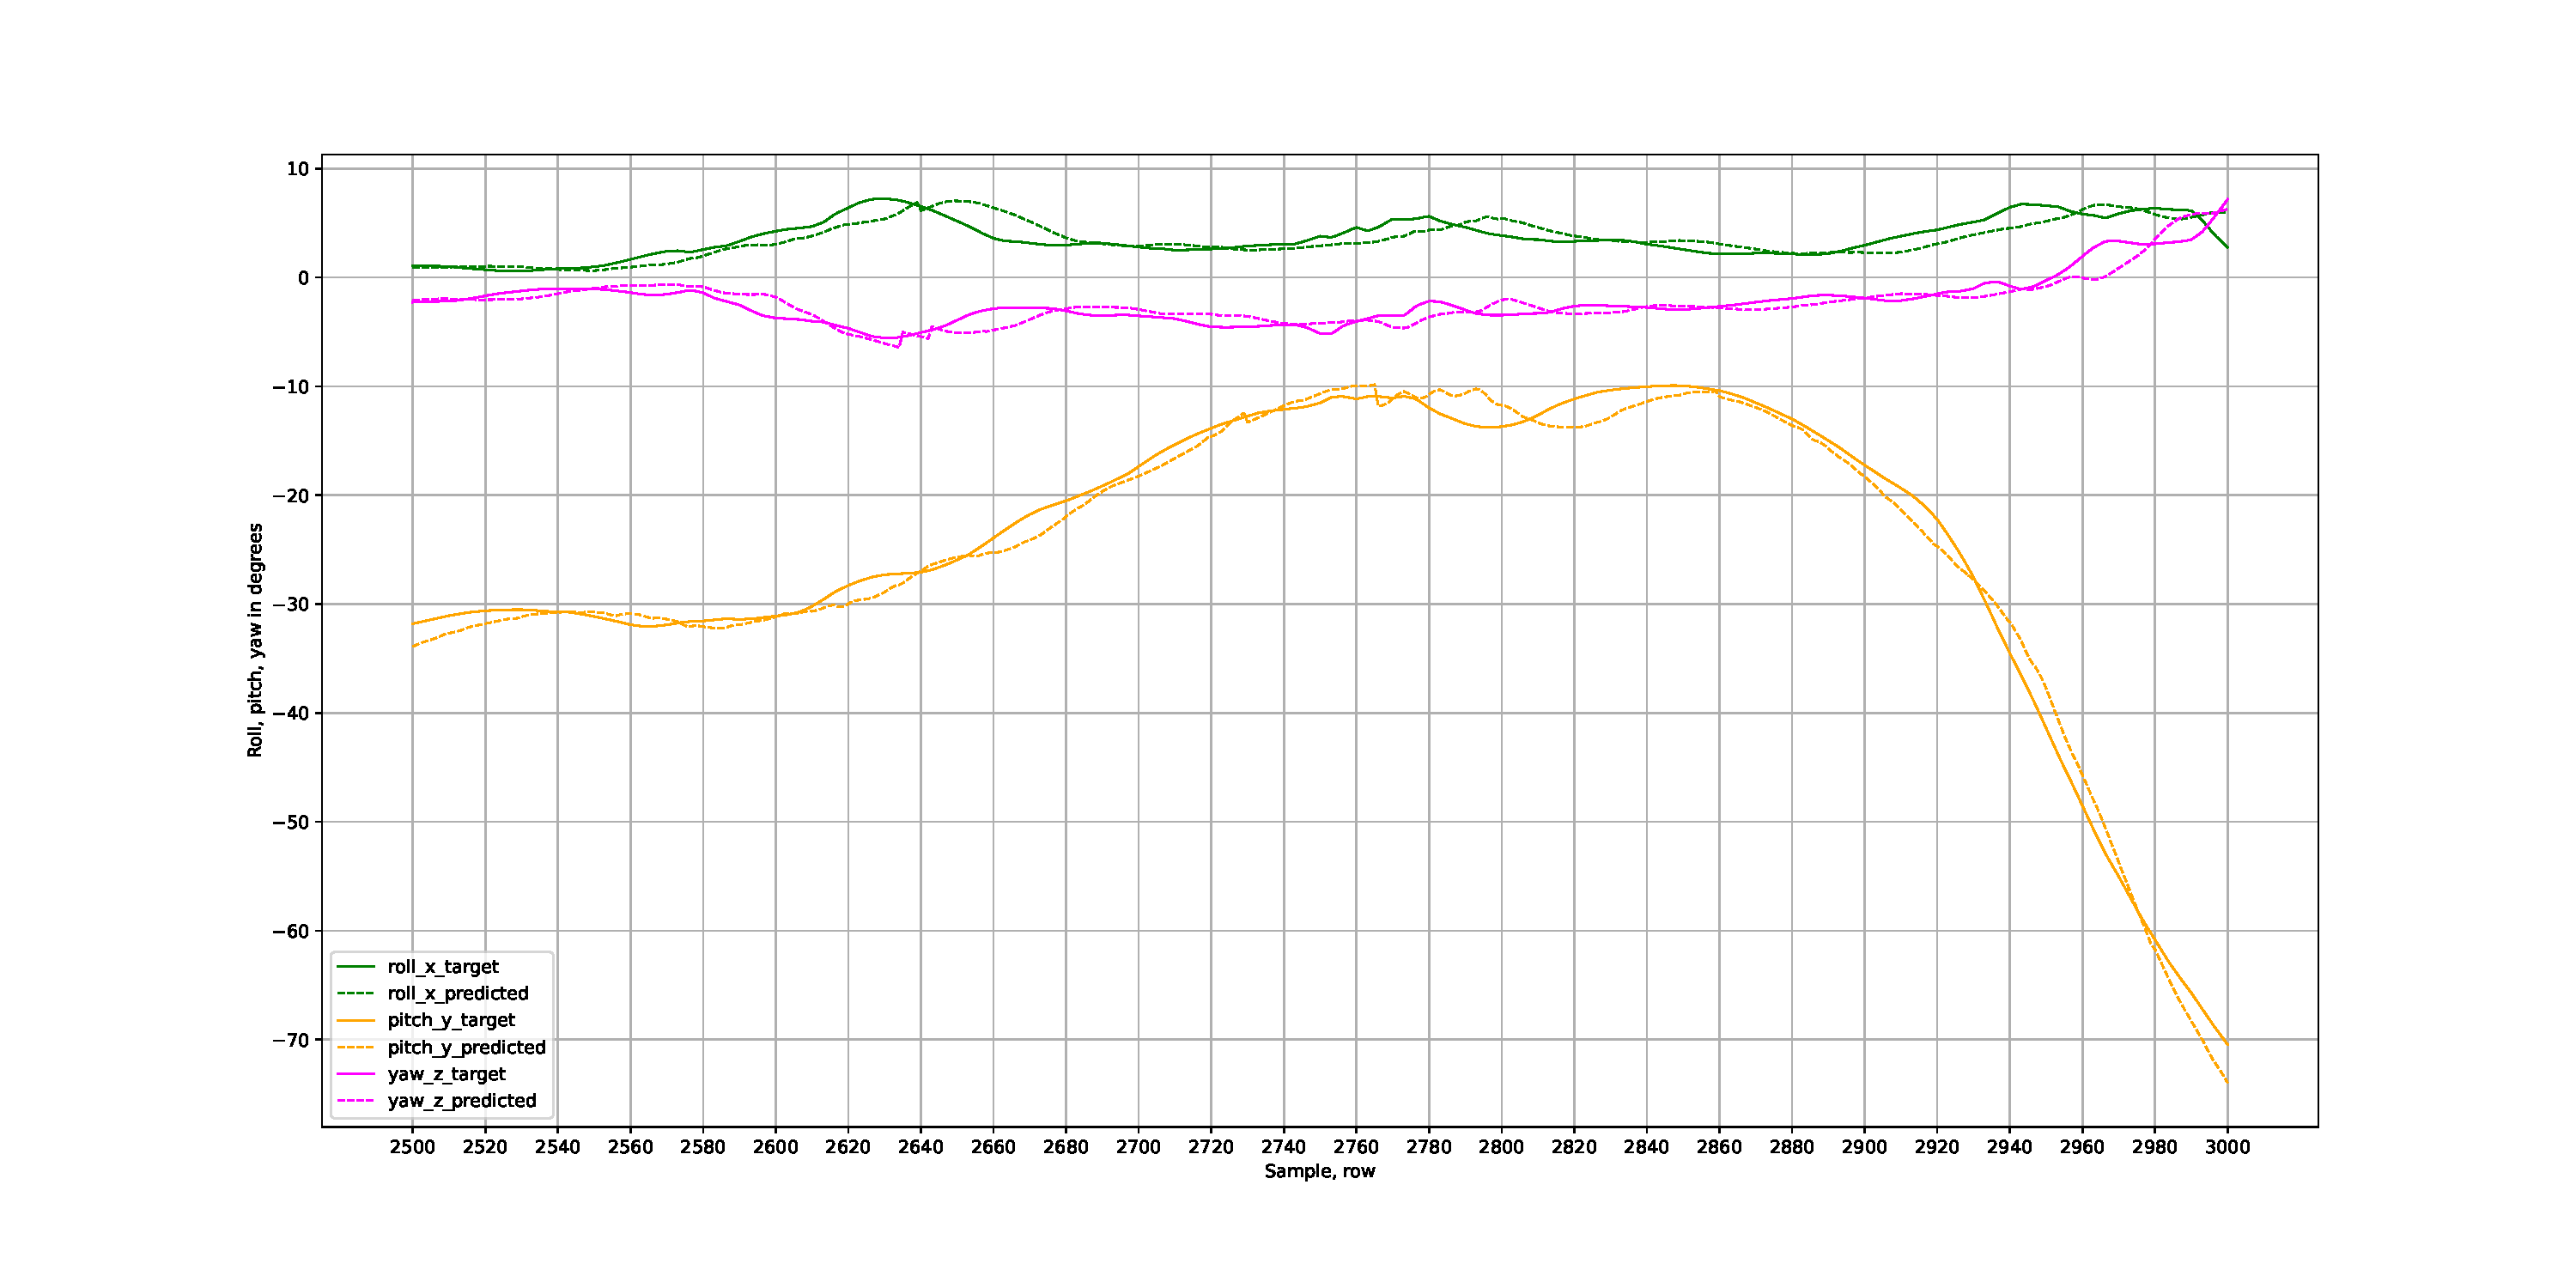
\includegraphics[width=0.8\textwidth, keepaspectratio]{gfx/gru1-roll_pitch_yaw_accuracy.pdf}
		\caption{GRU1 outputs for roll, pitch, yaw axes.}
		\label{fig:gru1-4}
	\end{center}
\end{figure}
In Fig. \ref{fig:gru1-4} illustrates the same 500 samples of rotational data. The evaluation metrics for rotation are still not low enough to allow predictions to exactly repeat the graph of real values. Compared to the results of LSTM1 on the full interpolated dataset with flipped negative quaternions, there is a visual improvement and reduction of the gap between the predicted- and real-graphs on the plotted range. Evaluation metrics for rotation are improved and root mean squared error significantly decreased. The square operation is applied to the mean error and thus $RMSE$ penalises bigger errors. It can be said that GRU1 rotational predictions have less outliers with higher distance to real data.

\subsection{Prediction with Bidirectional GRU}
\label{sec:eval:experiments:bi-gru}
The bidirectional GRU was evaluated as the last RNN variant. The goal of this evaluation is to check whether the bidirectional GRU will perform on a 6-DoF HoloLens dataset similar as is described in the section \ref{sec:related:deep}. Indeed, experiments showed that bidirectional GRU predicts worse than its unidirectional variant and even worse as the LSTM model. The best result that Bi-GRU can produce after 500 epochs of training with 1024 hidden dimensions is only twice better for position than an output of a Baseline model. However the rotation predictions are even worse that a Baseline outputs.The best metrics are as follows: $MAE_{pos} = 0.030$m, $RMSE_{pos} = 0.041$m, $MAE_{rot} = 30,19^{\circ}$ and $RMSE_{rot}  =33.78^{\circ}$. Fig. \ref{fig:grubi} shows the best prediction Bi-GRU could produce for a rotation and it is clear that the distance between real measured and predicted data is too significant to be able to consider these results as good. The similar behaviour is obtained for position but not plotted separately in the thesis. Additionally, Bi-GRU training took longer on GPU Cluster due the doubled hidden dimension size and on a local machine it is impossible to run the algorithm and get results in reasonable time. 
\begin{figure}[h!]
	\begin{center}
		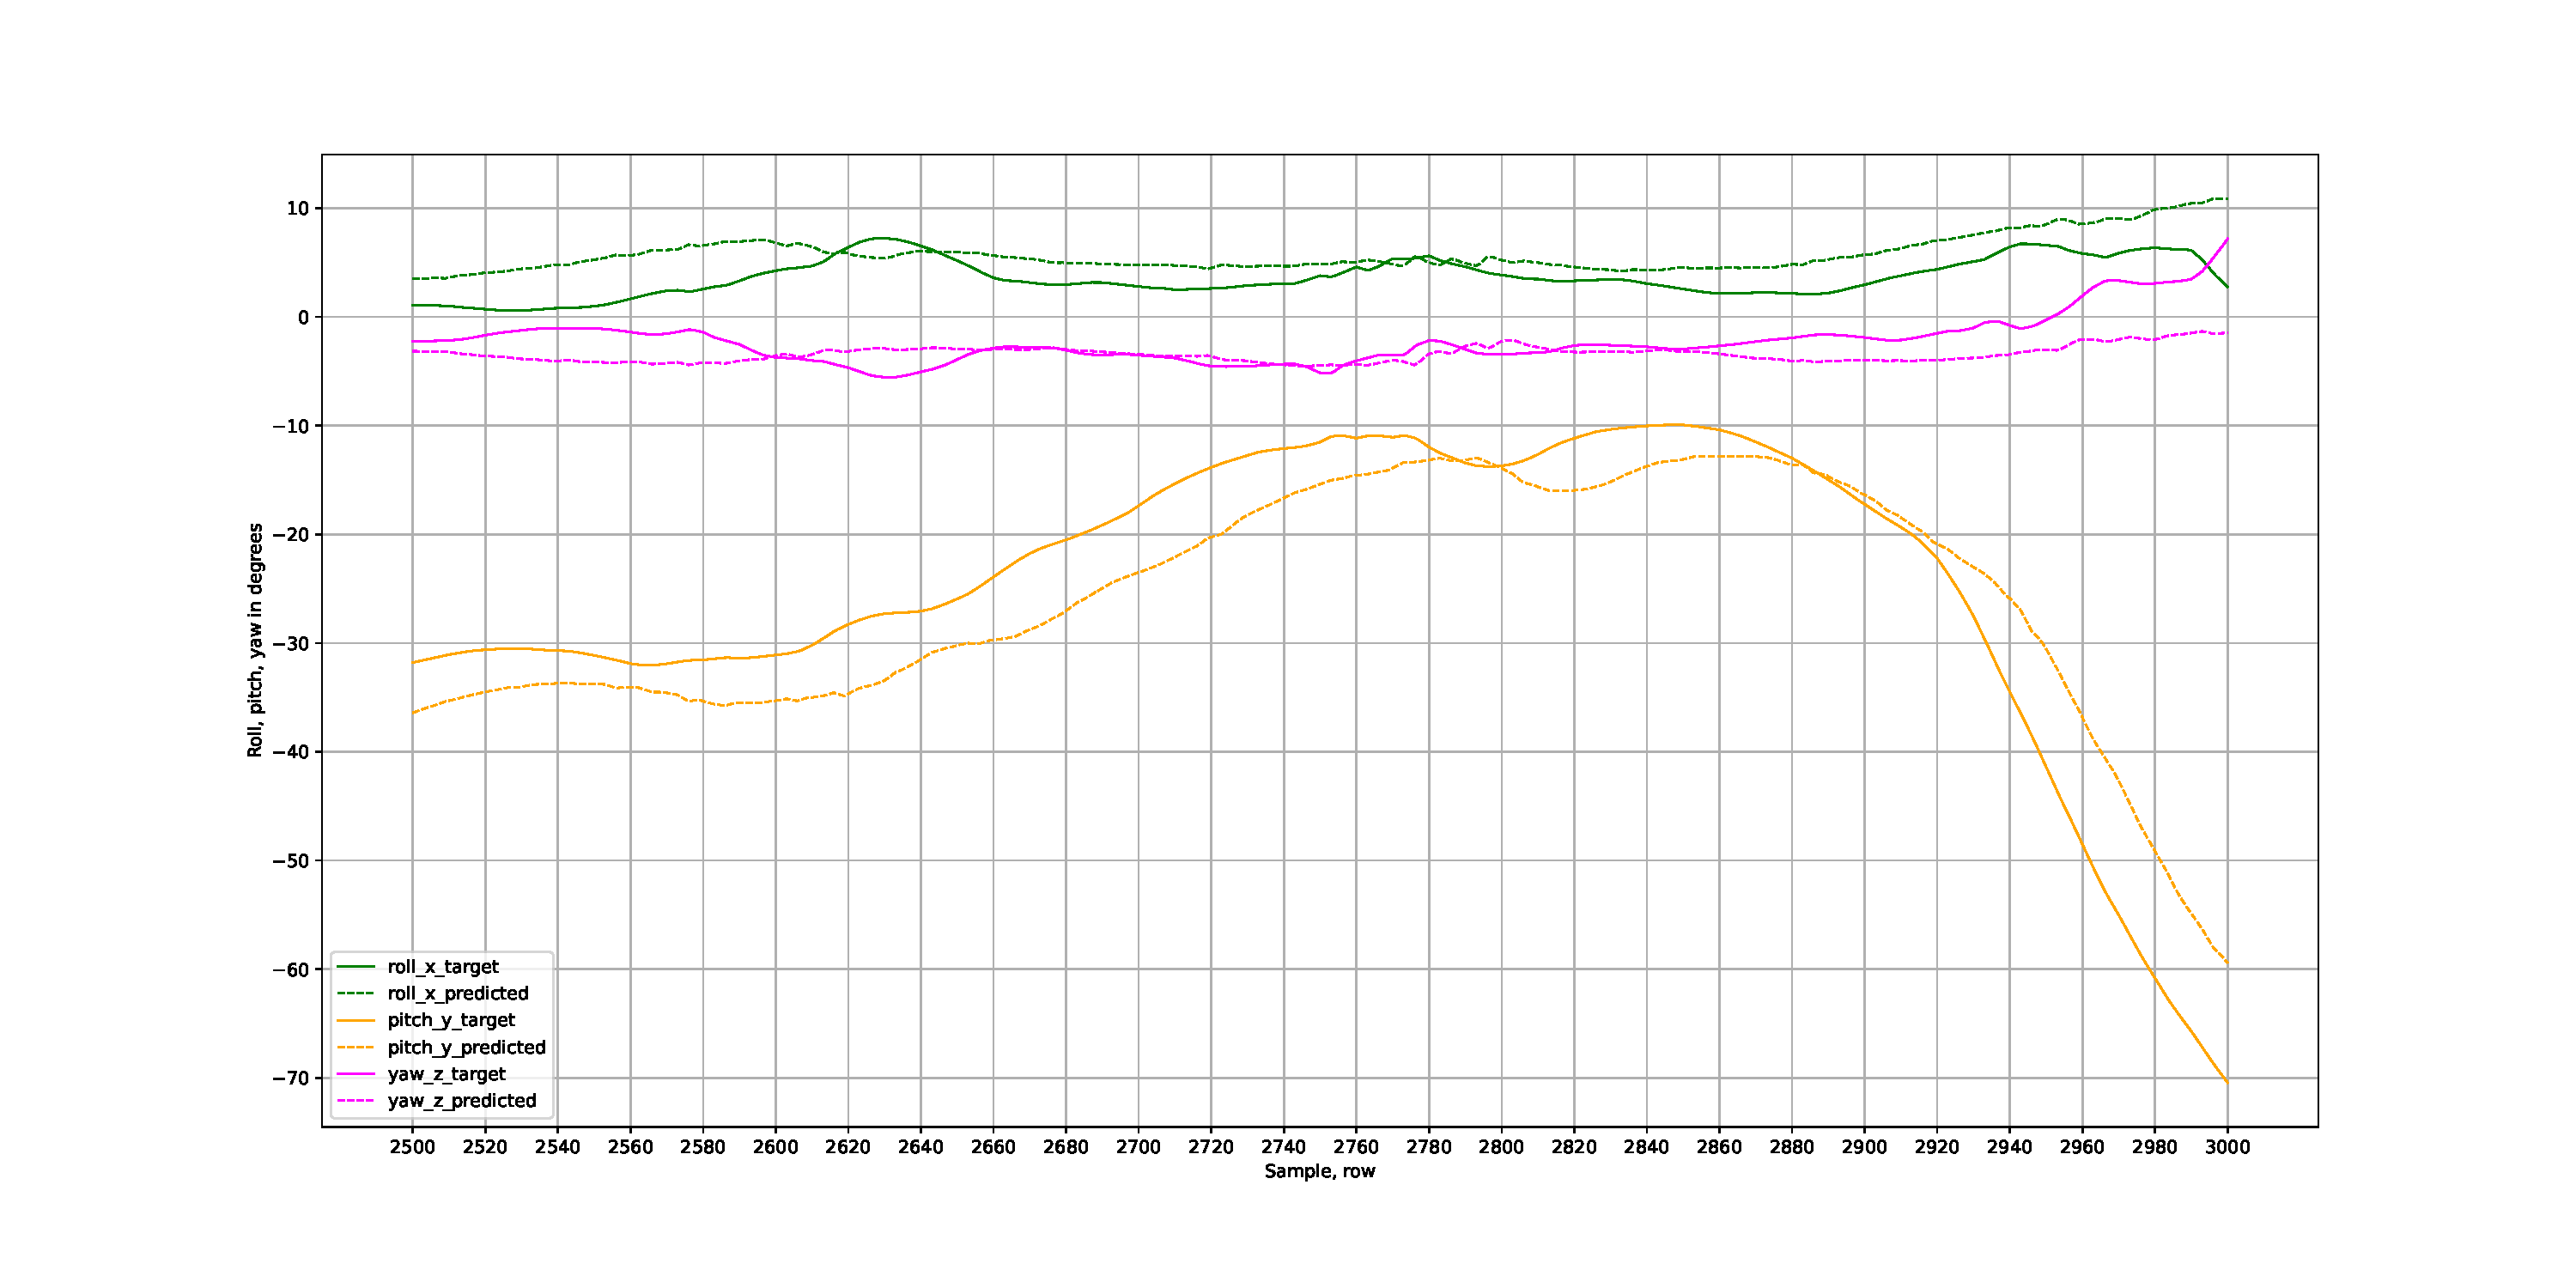
\includegraphics[width=0.7\textwidth, keepaspectratio]{gfx/gru-bi1-roll_pitch_yaw.pdf}
		\caption{Bidirectional GRU outputs for roll, pitch, yaw axes.}
		\label{fig:grubi}
	\end{center}
\end{figure}